% !Mode:: "TeX:UTF-8"
\documentclass[fontsize=11pt,a4paper,openleft,pagesize=auto]{book}
%\usepackage[scheme=chinese,9pt,heading]{ctex}
\usepackage{pifont}
%\usepackage{fontawesome}
\usepackage{fontspec}
%\usepackage[T1]{fontenc}
\usepackage{amsmath}
\usepackage{amssymb}
\usepackage{bm}
\usepackage{array}
\usepackage{enumitem}
\usepackage{imakeidx}
\usepackage[numbers,sort&compress]{natbib}
%\usepackage
%[paperheight=26 true cm,paperwidth=18.4 true cm,
%top=2.6 true cm,bottom=2.2 true cm,left=2.8 true cm,right=2.8 true cm]
%{geometry}
\usepackage{float}
%\usepackage{setspace}
\usepackage{hyperref}
\usepackage{bookmark}
\usepackage{caption}
%\usepackage[perpage,symbol*, bottom,hang,stable,multiple]{footmisc}
\usepackage[clearempty,pagestyles]{titlesec}
\usepackage{titletoc}
\titlecontents{section}[0pt]{\addvspace{2pt}\filright}
{\contentspush{\thecontentslabel\ }}
{}{\titlerule*[8pt]{.}\contentspage}
\usepackage[cmyk,table,hyperref]{xcolor}
\usepackage{tikz}
\usepackage{tcolorbox}
\usepackage{algorithm2e}
\usepackage{listings}
\usepackage{booktabs}
\usepackage{longtable}
\usepackage{makecell}
\usepackage{tabu}
\usepackage{mdframed}
\usepackage{pdfpages}
\usepackage{qrcode}
\usepackage{threeparttable}
%\usepackage{chngcntr}
\usepackage[nottoc,chapter]{tocbibind}
\AtEndPreamble{
	\usepackage[nohyphen,strings]{underscore}
}
\usepackage{lipsum}
\usepackage{graphicx}
%
% .:: footmisc ::.
%
% Circled Digit,带圆圈数字
%\DefineFNsymbols{cd}{{\ding{172}}{\ding{173}}{\ding{174}}{\ding{175}}{\ding{176}}{\ding{177}}{\ding{178}}{\ding{179}}{\ding{180}}{\ding{181}}}
%% Negative Circled Digit,反白带圆圈数字
%\DefineFNsymbols{ncd}{{\ding{182}}{\ding{183}}{\ding{184}}{\ding{185}}{\ding{186}}{\ding{187}}{\ding{188}}{\ding{189}}{\ding{190}}{\ding{191}}}
%% Circled Sans-Serif Digit,带圆圈无衬线数字
%\DefineFNsymbols{cssd}{{\ding{192}}{\ding{193}}{\ding{194}}{\ding{195}}{\ding{196}}{\ding{197}}{\ding{198}}{\ding{199}}{\ding{200}}{\ding{201}}}
%% Negative Circled Sans-Serif Digit,反白带圆圈无衬线数字
%\DefineFNsymbols{ncssd}{{\ding{202}}{\ding{203}}{\ding{204}}{\ding{205}}{\ding{206}}{\ding{207}}{\ding{208}}{\ding{209}}{\ding{210}}{\ding{211}}}
%\setfnsymbol{cssd}
%\setlength\footnotemargin{.6em}

% package: float
\floatplacement{figure}{!ht}

% package: booktab
%\setlength\aboverulesep{0sp}
%\setlength\belowrulesep{0sp}
%\setlength\cmidrulesep{0sp}

% package: graphicx
\graphicspath{{resources/}}

% package: caption
%\DeclareCaptionFont{31104}{\FZYZK}
%\captionsetup{format=hang,labelsep=quad,font=31104}
%\DeclareCaptionFormat{31104}{%
%%	\bfseries\footnotesize#3
%\footnotesize#3
%}
%\captionsetup[lstlisting]{format=31104,singlelinecheck=off}

% package: enumitem
%\setlist{noitemsep,partopsep=0pt}%,listparindent=\parindent
%\setlist[1]{labelindent=\parindent}
%\setlist[itemize]{topsep=0pt,parsep=.5\parskip,leftmargin=1.5em}
%\setlist[itemize]{topsep=0pt,parsep=.5\parskip,leftmargin=3.5em}
%\setlist[enumerate]{topsep=0pt,parsep=.5\parskip,labelsep=*,leftmargin=1.5em}
%\setlist[enumerate,1]{topsep=0pt,parsep=.5\parskip,labelsep=*,leftmargin=3.5em}
%\setlist[description]{topsep=0pt,parsep=.5\parskip,labelsep=.25em,leftmargin=*}

% 图表编号分隔符
\makeatletter
\renewcommand\thefigure{\ifnum \c@chapter>\z@ \thechapter -\fi \@arabic\c@figure}
\renewcommand\thetable{\ifnum \c@chapter>\z@ \thechapter -\fi \@arabic\c@table}
\makeatother

% 以下设置正文字体为 Palatino 的克隆体
\setmainfont{TeX Gyre Termes}
% 以下设置等宽字体为 Courier 的克隆体
\setmonofont{Monaco}

% 代码风格
\lstset{ %
	language=C++,                % the language of the code
	basicstyle=\scriptsize \fontspec{Monaco},           % the size of the fonts that are used for the code
%	basicstyle=\scriptsize \ttfamily
	numbers=left,                   % where to put the line-numbers
	numberstyle=\tiny\color{gray},  % the style that is used for the line-numbers
%	% will be numbered
	numbersep=5pt,                  % how far the line-numbers are from the code
	showspaces=false,               % show spaces adding particular underscores
	showstringspaces=false,         % underline spaces within strings
%	showtabs=false,                 % show tabs within strings adding particular underscores
	frame=shadowbox,                   % adds a frame around the code
%	%	rulecolor=\color{black},        % if not set, the frame-color may be changed on line-breaks within not-black text (e.g. commens (green here))
	tabsize=2,                      % sets default tabsize to 2 spaces
	%	captionpos=b,                   % sets the caption-position to bottom
	breaklines=true,                % sets automatic line breaking
%	breakatwhitespace=false,        % sets if automatic breaks should only happen at whitespace
%	title=\lstname,                   % show the filename of files included with \lstinputlisting;
	% also try caption instead of title
	keywordstyle=\color{blue!60},          % keyword style
	rulesepcolor=\color{blue!20},%
	commentstyle=\color{gray}, %
}

% 目录双栏
%\usepackage{multicol}
%\makeatletter
%\renewcommand\tableofcontents{%
%	\begin{multicols}{2}[%
%		\section*{%
%			\contentsname
%			\@mkboth{\MakeUppercase\contentsname}{\MakeUppercase\contentsname}}]%
%		\@starttoc{toc}%
%\end{multicols}}
%\makeatother


\makeatletter

\providecommand\optional{\stepcounter{enumi}\labelenumi\makebox[0pt][l]{$^*$}}

% +----------------------------------------------+
% : 重定义                                       :
% +----------------------------------------------+
\renewcommand{\figureautorefname}{\figurename}
\renewcommand{\tableautorefname}{\tablename}


% +----------------------------------------------+
% : 废弃命令                                     :
% +----------------------------------------------+
\def\tightlist{}

% +----------------------------------------------+
% : 取消篇标题单独页                             :
% +----------------------------------------------+
\def\@endpart{}

% +----------------------------------------------+
% : PDF属性设置                                  :
% +----------------------------------------------+
\AtEndPreamble{
	\hypersetup{
		pdfinfo={
			Title    = {\@title},
			Author   = {\@author},
			Creator  = {Adobe Acrobat 11.0},
			Producer = {Acrobat Web Capture 11.0}
		}
	}
}

% +----------------------------------------------+
% : tex.stackexchange.com/a/40363                :
% +----------------------------------------------+
\patchcmd{\@addtocurcol}%
	{\vskip \intextsep}%
	{\edef\save@first@penalty{\the\lastpenalty}\unpenalty
		\ifnum \lastpenalty = \@M % hopefully the OR penalty
			\unpenalty
		\else
			\penalty \save@first@penalty \relax % put it back
		\fi
		\ifnum \outputpenalty <-\@Mii
			\addvspace\intextsep
			\vskip\parskip
		\else
			\addvspace\intextsep
		\fi}%
	{\typeout{*** SUCCESS ***}}{\typeout{*** FAIL ***}}

\patchcmd{\@addtocurcol}%
	{\vskip\intextsep
		\ifnum \outputpenalty <-\@Mii
			\vskip -\parskip
		\fi}%
	{\ifnum \outputpenalty <-\@Mii
		\aftergroup\vskip\aftergroup\intextsep
		\aftergroup\nointerlineskip
	\else
		\vskip\intextsep
	\fi}% was the float seen in vertical mode?
	{\typeout{*** SUCCESS ***}}{\typeout{*** FAIL ***}}

\patchcmd{\@getpen}{\@M}{\@Mi}
	{\typeout{*** SUCCESS ***}}{\typeout{*** FAIL ***}}

% +----------------------------------------------+
% : Verbatim callouts                            :
% +----------------------------------------------+

% Counters for cross-referencing callouts
\newcounter{cocnt}
\newcounter{colref}

% How to represent the <co> markup.
% Big thanks to Jean-Côme Charpentier for his help.
%
\newlength{\co@width}
\newlength{\co@height}
\newlength{\balldiam}
\newlength{\ballcentre}
\newlength{\ballcenter}% 修正纵向位置

\def\conum#1{%
	\sbox{\z@}{\color{white}\sffamily\bfseries\tiny#1}% 
	% Box sizes for any number with two digits
	\sbox{\@ne}{\color{white}\sffamily\bfseries\tiny00}%
	\settowidth{\co@width}{\usebox{\@ne}}%
	\settoheight{\co@height}{\usebox{\@ne}}%
	% Find out the biggest length, to define the circle diameter
	\ifnum\co@width>\co@height
		\setlength{\balldiam}{\co@width}%
	\else
		\setlength{\balldiam}{\co@height}%
	\fi
	\balldiam=1.45\balldiam
	\ballcentre=0.5\balldiam
	\ballcenter=0.3\balldiam% 修正纵向位置
	\setlength{\unitlength}{1pt}% In the case it has been changed
	\begin{picture}(\strip@pt\balldiam,\strip@pt\balldiam) %
	\put(\strip@pt\ballcentre,\strip@pt\ballcenter){\circle*{\strip@pt\balldiam}}
	\put(\strip@pt\ballcentre,\strip@pt\ballcenter){\makebox(0,0){\usebox{\z@}}}
	\end{picture}%
}

% How to represent a <co> embedded in a listing
\def\co#1{\refstepcounter{cocnt}\conum{#1}}

% Make the <co> text and the label to link to
\def\coref#1#2{\co{#1}\label{#2}}

% Make only the <co> label to link to
\def\colabel#1{\refstepcounter{cocnt}\label{#1}}

% Make the <callout> label to link to
\def\collabel#1{\refstepcounter{colref}\label{#1}}

\makeatother


% suggested format in Springer
%i.Title page
%ii.Author details and  Springer copyright page
%iii.Dedication page
%iv.Acknowledgments
%v.Preface
%vi.Table of contents
%vii.Introduction

\begin{document}
% Title page
\title{SLAM in Robotics and Autonumous Driving}
\author{Xiang Gao}
\date{Last update: \today}

\frontmatter
\maketitle

% section starts from 1
\makeatletter
\@addtoreset{equation}{section}
\makeatother

% Author info & copy right

% dedication page
\clearpage
\begin{center}
	\thispagestyle{empty}
	\vspace*{\fill}
	\usefont{T1}{LobsterTwo-LF}{bx}{it}
	\Large \emph{To my beloved Lilian and Shenghan}
	\vspace*{\fill}
\end{center}

\tableofcontents

\thispagestyle{empty}
%!Mode:: "TeX:UTF-8"
\thispagestyle{empty}
\chapter*{Preface}
\thispagestyle{empty}
\section*{About this book}

Well, autonomous driving is a such cool stuff, isn't it? 

You've probably seen scenes of self-driving cars in science fiction movies. In these vehicles, the steering wheel turns by itself, the throttle and brakes are controlled automatically, freeing people from the monotony of driving so they can enjoy their time more freely. In fact, some Level 2 vehicles have already achieved partial self-driving capabilities in simple road conditions. They can help drivers keep the vehicle centered in the lane or maintain a certain distance from the preceding vehicle. These systems are called \textbf{Advanced Driver Assistance Systems (ADAS)}. And for more advanced self-driving systems (Level 4), computers can fully take over, not only assisting drivers but also controlling buses, delivery vehicles, robots, robotic dogs, and even bicycles, enabling many functionalities we never imagined. Over time, these sci-fi-like scenes have gradually become reality. Self-driving jobs have also emerged as a new industry, attracting young talents from all sectors of society. It's truly an exciting development!

The field of autonomous driving encompasses many emerging technologies, with Simultaneous Localization and Mapping (SLAM) being a key focus. Since completing my PhD, I have been involved in the research and development of SLAM in the autonomous driving industry. It's an intriguing area because whether it's large passenger vehicles, small low-speed vehicles, or even sweepers, SLAM is certainly a fundamental technology. Most of the automation features we see are actually embedded within the vehicle's map data. For instance, the map might instruct the vehicle to turn left at the upcoming intersection and merge into the right lane of the opposite road; or, for cleaning a plaza ahead, the vehicle should drive along the right boundary in circles while avoiding the flower bed area in the middle. To achieve these functionalities, we need to integrate various types of data such as GPS, inertial navigation, laser point clouds, visual images, etc., to construct maps and then perform localization on these maps.

If you work in this area, you'll find that it brings together people with diverse backgrounds. People working on inertial navigation are familiar with strapdown inertial navigation systems. They enjoy writing matrix and vector computation programs on a small embedded CPU, often scratching their heads over errors of one or two points aboue accuracy. Those involved in processing laser point clouds engage in meticulous map reconstruction, displaying beautiful three-dimensional point clouds on the screen. Meanwhile, those working on vision spend their days manipulating images on the imaging plane, producing impressive results but not focusing much on accuracy issues. Well, I mean, accuracy is of course an important issue, but the accuracy on a two-dimensional imaging plane is not the same as the accuracy of three-dimensional world points or localization accuracy. Cameras usually don't have fixed accuracy metrics like other sensors. They can either focus on nearby objects for local high precision or distant objects for a broad field of view, just like the difference between a microscope and a telescope. Thanks to the collaboration among these individuals and effective communication from management, vehicles are able to navigate the roads stably. However, most of the time, we aren't entirely clear about what other people are doing or how they're doing it. This is one of the motivations for me to write this book.


I hope to introduce readers to the localization and mapping technologies related to autonomous driving and robotics in this book, which include the sensors we use in our daily lives. Although there is currently no unified opinion on what constitutes a vehicle or a robot, they can even be seen as wheeled smartphones. However, these intelligent machines all use similar sensors, and the underlying theories are basically the same. I hope that through this book, researchers in this field can enhance mutual understanding, or colleagues and students outside the field can understand what work we are doing. I believe many people will be interested in these technologies.

\subsection*{Content of This Book}
This book introduces SLAM-related technologies used in autonomous driving and robotics. The SLAM discussed here is quite general. We will cover sensors and processing methods related to localization and mapping. A typical autonomous vehicle will include various sensors such as IMU, wheel encoders, vehicle speed sensors, and multi-line laser sensors, so our localization and mapping will also involve methods for these sensors. Therefore, readers will encounter topics like basic algorithms for inertial navigation, filters represented by Kalman filtering, laser point cloud matching methods, trajectory fusion algorithms, and more in this book. Overall, we will introduce these contents in the following order:

\begin{enumerate}
	\item The first part covers \textbf{Basic Mathematical Knowledge}. We will start with basic coordinate system definitions, rotational geometry, and quickly introduce some mathematical background knowledge used in this book. Since most of this background knowledge can be found in other books and materials, we will only provide a brief introduction. Chapter 1 of Part 1 provides an overview of autonomous driving, Chapter 2 introduces basic geometry and kinematics, Chapter 3 covers the error Kalman filter used for integrated navigation, and Chapter 4 introduces pre-integration systems and optimization methods. Readers don't need to worry about the specialized terminology mentioned here; we will delve into them in detail in specific chapters.
	\item The second part is about \textbf{Laser Localization and Mapping}. This section introduces 2D and 3D laser localization technologies, with the former mainly used in robots represented by sweepers, and the latter being one of the foundational technologies for autonomous driving vehicles. We will detail representative techniques for processing laser point clouds and demonstrate their applications through code implementation. Chapter 5 of Part 2 introduces basic point cloud processing algorithms (nearest neighbor structures, KD trees, etc.), Chapter 6 discusses 2D laser localization and mapping, and Chapter 7 covers 3D laser localization and mapping.
	\item The third part focuses on \textbf{Application}. We will discuss the process of building high-precision point cloud maps for autonomous driving and how to use point cloud maps for real-time localization. Chapter 8 introduces tightly coupled laser-inertial odometry methods, Chapter 9 presents offline point cloud mapping systems, and Chapter 10 introduces online fusion localization systems.
\end{enumerate}

Similar to my previous book\footnote{\url{https://github.com/gaoxiang12/slambook-en}}, this book emphasizes the unity of theory and practice and pays close attention to the implementation of principles in code. All algorithms mentioned in this book will have code implementations provided in the corresponding chapters. Readers will work with us to implement those important and foundational algorithmic structures in this field from scratch, using modern programming techniques and fully exploiting parallelization principles to make our algorithms run smoother than classical implementations. Consequently, we will not limit ourselves to specific implementations of open-source code. For example, we will avoid discussing what LOAM does from line X to line Y or which library Cartographer references in a particular cpp file. We will refrain from discussing engineering details like thread pools or parameter file formats. Yes, such discussions can be too detailed, and everyone's implementation may differ. We will strive to retain only the core algorithmic code, allowing readers to debug and understand the entire process themselves.

In terms of style, I will continue to use my familiar writing style. Readers who are familiar with me should quickly adapt, while those who are not should not find it overly challenging. I hope my writing is as clear and straightforward as a conversation. Throughout the introduction of content, I hope the reading process reflects a complete train of thought, rather than simply compiling information together. Although this writing style may result in some verbosity, I believe it is beneficial.

\textbf{The majority of the key contents in this book will be accompanied by corresponding implementation code}. This is one of the major features of this book. I believe that for a comprehensive book, providing code that demonstrates the concepts is always a wise choice. However, despite our efforts to streamline the code, the code section of this book is still much larger than my previous book.

Here is our code repository:

\begin{mdframed}
	\centering
	\url{https://github.com/gaoxiang12/slam_in_autonomous_driving}
\end{mdframed}

Please checkout the "en" branch if you only want to read English comments.

All code and data for this book are open-source and freely accessible to readers. The PDF file of this book will be continuously updated within the code repository. We use C++ as the primary programming language. Please don't ask me why I didn't use more concise languages like Python or Matlab because the programs running in actual vehicles or robots are still primarily C++ programs, and I don't want our experiments to deviate too far from industrial applications. Please note that the code, errata, and other files for this book will be updated on GitHub first, while the published version of the book may have a certain lag time due to the printing schedule of the publishing house. If readers find any discrepancies between the content in the book and the code repository, please consider the implementation in the code repository as authoritative.

We welcome readers to ask questions or answer questions from other readers in the code repository of this book. We encourage readers to communicate in English to facilitate sharing your experiences with international friends.

\subsection*{How to Use This Book}
The content of this book follows a process of gradually deepening complexity, but even basic topics like those in Chapter 2 require some groundwork. Personally, I hope this book serves as a sequel to my previous book \cite{Gao2017} (\url{https://github.com/gaoxiang12/slambook-en}). You should at least read the first 6 chapters of that book to familiarize yourself with some basic mathematical principles and the basic usage of optimization libraries. However, if readers have not read that book, you should at least have knowledge in the following areas:

\begin{itemize}
	\item Basic undergraduate-level mathematics such as calculus, linear algebra, and probability theory.
	\item Mathematics at the graduate level: optimization, matrix theory, a small amount of knowledge about Lie groups and Lie algebras.
	\item Computer science: Linux system operations, C++ programming language.
\end{itemize}

If readers find certain parts of this book difficult to understand, they can refer to corresponding reference books for supplementary learning. Overall, this book will be slightly more challenging and the pace of introduction will be somewhat faster.

The code for this book is organized by chapter. For example, the code for Chapter 3 will be located in src/ch3. The code for each chapter will be compiled into separate library files and executable files. Additionally, shared code will be placed in src/common (such as some common structures, message definitions, UI, etc.). There is a certain degree of dependency between the code of different chapters, with later chapters reusing the results of earlier chapters. The code for this book needs to be compiled using ROS, but the actual running and testing processes do not require the use of ROS mechanisms; only ROS data packages are used for storage. Readers only need to understand the installation process of ROS and do not need to familiarize themselves with the details of ROS in advance.

\subsection*{Notations}
The mathematical symbols in this book follow the international standard. In general, scalars are expressed in slanted font, such as $a$; matrices and vectors are represented in bold font, such as $\mathbf{A}$; special sets are denoted in hollow sans-serif font, such as $\mathbb{R}$; and Lie algebra-related sets are expressed in Gothic font, such as $\mathfrak{so}(3)$. We aim to maintain consistency throughout the book in terms of symbols, with additional explanations provided where ambiguity may arise.

\subsection*{Relationship with Other Books and Papers}
Autonomous driving localization technology involves many active research fields. For example, Professor Barfoot's "State Estimation for Robotics" \cite{Barfoot2016} focuses on introducing state estimation theory. Its Chinese translation was also translated by our team. On the one hand, it provides a comparative introduction to the differences and similarities between traditional filtering theory and modern optimization theory, and on the other hand, it provides an excellent introduction to Lie groups and Lie algebra for engineering readers. This book will partially use some conclusions from the book on state estimation, mainly the part related to Lie groups and Lie algebras, to support some of our formula derivations.

Professor Ma's "An invitation to 3-d vision: from images to geometric models" \cite{Ma2012a} is also an excellent book that introduces knowledge of 3D vision, with many similarities in the basic knowledge of 3D geometry.

Joan Sol{\`{a}}'s "Error State Kalman Filter" \cite{Sola2017} provides a very concise and precise theory of quaternion-based error Kalman filters. Although it is not lengthy, it discusses quaternions and Kalman filters very thoroughly, and most derivations in this field are based on this material. This book will also use some of its results, but we will mainly derive various filter formulas based on Lie groups rather than quaternion forms.

Professor Thrun's "Probabilistic Robotics" \cite{Thrun2005} is also a well-known classic book in the field of robotics. It introduces some results related to SLAM in the field of robotics, and provides a very detailed introduction to traditional filters, 2D grid maps, and other content. This book will also introduce 2D grid localization and mapping methods, with the theoretical part also referencing this book's content.

Professor Qin Yongyuan and Professor Yan Gongmin's works in the field of inertial navigation, including "Inertial Navigation" \cite{Qin2014}, "Kalman Filter Algorithm and Combination Navigation Principle for Strapdown Inertial Navigation" \cite{Yan2019}, and "Inertial Instrument Testing and Data Analysis" \cite{Yan2012}, are classic textbooks in this field, and many teachers and students studying inertial navigation will refer to their derivation process. This book also refers to these books in the field of inertial navigation, but compared to specialized textbooks on inertial navigation, the content introduced in this book will be relatively basic. We mainly introduce the basic principles of inertial navigation, without involving complex parameter compensation or discussions on various subdivided motion states. However, in contrast, the preintegration principle and nonlinear optimization part introduced in this book are not fully introduced in these traditional textbooks.

Finally, compared to the books and materials mentioned above, the biggest feature of this book is still the unity of code and theory. It can be said that most books are for reading, while this book can be \textbf{executed}. I believe that understanding many algorithmic aspects requires readers to participate in the debugging and running process.

\subsection*{Environment}
This book uses Ubuntu 20.04 as the experimental environment. Readers can use their personal computers as development environments. If familiar with Docker, they can also use Docker environments. The book primarily utilizes \textbf{C++17} as the C++ standard, which may be relatively new to some readers. Older machines or environments may not necessarily support it well. We recommend readers to use software environments above Ubuntu 20.04 to run the code in this book; otherwise, you may need to address some minor issues regarding C++ standard support.

This book comes with a considerable amount of test data, which is quite large (approximately 270GB). We suggest that readers allocate at least 100GB of space to run the code in this book. Readers can download the test data through the links provided in the book's repository.

\subsection*{Acknowledgement}
\begin{enumerate}
	\item Considering the confidentiality of geographical information, this book avoids using domestic data and tends to use open-source datasets worldwide. Readers can consider the trajectories or point clouds provided in the book as data in a general spatial coordinate system, without concerning themselves with the actual geographical locations of this data.
	\item Similarly, unless necessary, the data provided in this book will not specify geographical information such as place names or ranges. Readers can regard them as general road, plaza, or building scenes.
	\item Some of the images used in this book are sourced from internet search engines and are used solely for educational purposes, with no intention of infringing on the original authors' copyrights. Some of the images used in this book may contain logos of commercial companies or may be images used in promotional materials for some companies. These images are sourced from public search engines and do not imply any cooperation or competition relationship between the authors and the companies. The author will strive to obtain authorization for images that may have commercial copyrights. If there is any dispute, please inform us.
	\item Each chapter of this book uses datasets from different sources, mainly including the NCLT dataset from the University of Michigan \cite{CarlevarisBianco2015}, the UTBM dataset from Montbéliard, France \cite{Yan2020}, and the UrbanLoco dataset mainly from Hong Kong, China \cite{Wen2020} (ULHK), among others. This book has designed a unified interface for them programmatically, making it convenient for readers to test the performance of algorithms on different datasets.
	\item The English version of this book is translated with the help of ChatGPT and I would like to thank their great work here.
\end{enumerate}

\thispagestyle{empty}
\mainmatter

% 1. background
% !Mode:: "TeX:UTF-8"
% 本章介绍自动驾驶基础知识、高精地图作用与使用范围等等
\thispagestyle{empty}
\setcounter{page}{1}
\part{Basic Knowledge}
\thispagestyle{empty}
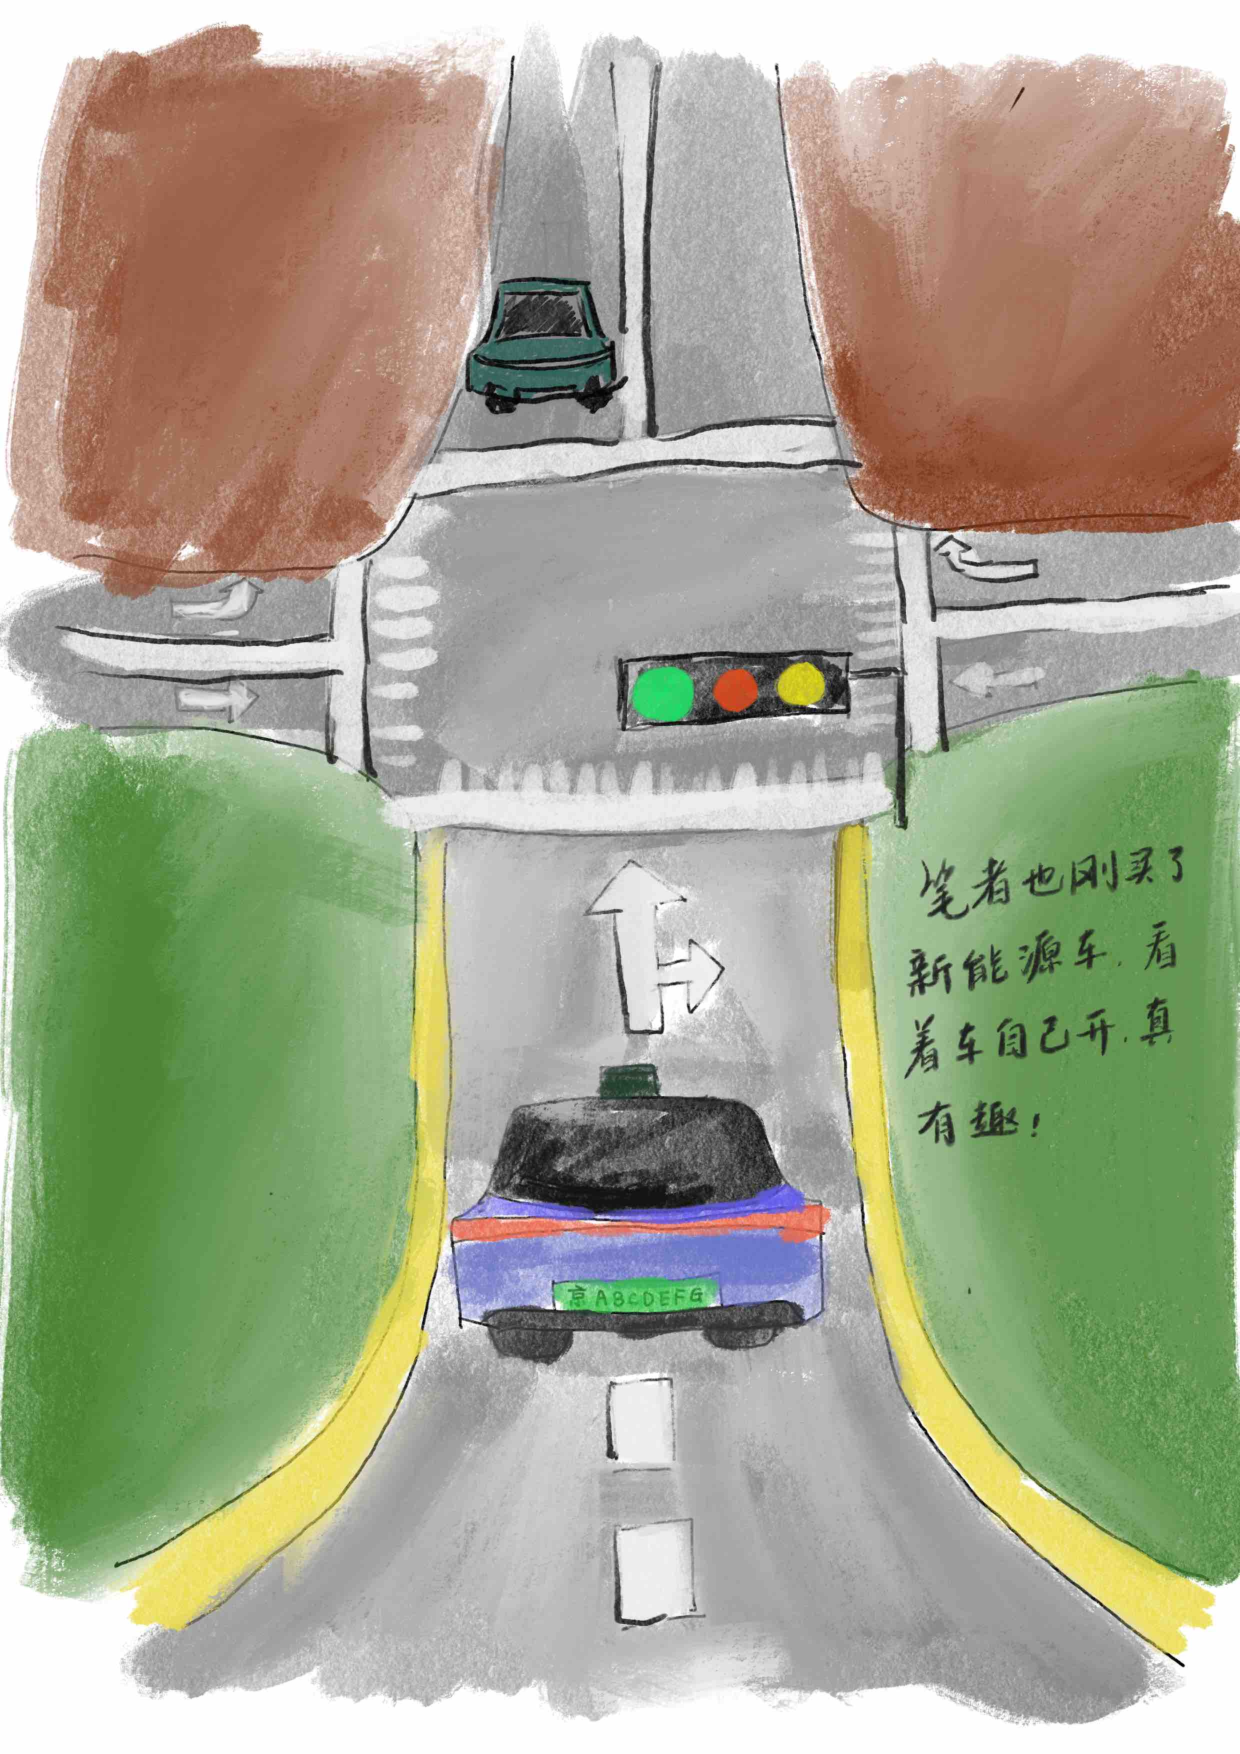
\includepdf[width=\textwidth]{art/ch1.pdf}

\newpage

\chapter{Autonomous Driving}
\thispagestyle{empty}
\setcounter{chapter}{1}
\section{Autonomous Driving Technologies}
\subsection{Autonomous Driving Capabilities and Grading}
Autonomous driving, as the name suggests, is the study of enabling vehicles to drive by itself. If you were to design an autonomous driving system, where would you start?

Although the internal structure of a car is highly complex, what humans actually need to operate is simply looking ahead, manipulating the steering wheel, accelerator, and brake pedals. If a computer program also learns to send signals to the steering wheel and pedals based on information from camera images, does it qualify as learning autonomous driving? If so, how should this program be designed?

In a naive conception, to enable a car to autonomously drive, one should first observe how humans perform driving behaviors. Humans primarily use vision to judge the relationships between their own vehicles and surrounding vehicles, pedestrians, and roads. They determine the direction of travel by observing lane markings and then use maps to determine long-term route planning. Similarly, autonomous vehicles should possess these abilities. Let's make a simple analogy:

\begin{enumerate}
	\item Autonomous vehicles should be able to identify the types of surrounding vehicles and pedestrians in real time, recognize road signs and signals, such as common lane markings, traffic lights, and traffic signs. This is called the \textbf{perception} capability of the vehicle \cite{Qian2020, Zhang2018}.
	\item The vehicle should be able to determine its own direction and position, as well as the positional relationship between itself and the aforementioned elements. This is also known as the \textbf{localization} capability of the vehicle \cite{Wei2020, Hungar2020, Wang2017}.
	\item The vehicle should be able to control the throttle, brake, steering wheel, and other actuators based on the aforementioned signal recognition results, and plan short-term and long-term driving routes. This is called the \textbf{planning and control} (P\&C) capability of the vehicle \cite{Sun2018, Viana2021}.
\end{enumerate}

However, despite addressing the same problems, the capabilities of humans and computers differ greatly. Throughout the long history of evolution, humans have developed extremely powerful spatial \textbf{perception} abilities. We can understand the vast majority of objects in our field of vision in an instant, with minimal errors. We also possess strong learning abilities; even when encountering unfamiliar objects, we instinctively avoid them. We can quickly understand the structure of the road ahead in any weather and scene, and even drive normally on roads without lane markings. We can also communicate with surrounding vehicles through lights and sounds, and predict their actions based on the behavior of other vehicles. In some defensive driving techniques, we can even infer potential dangers in blind spots. Due to these powerful understanding abilities, we can drive vehicles freely based solely on vision, without precise position and attitude information, unlike autonomous vehicles, which require expensive ranging devices like LiDAR, high-definition maps, and high-precision positioning to precisely control vehicle behavior (Figure \ref{fig:human-auto}).

\begin{figure}[!htp]
	\centering
	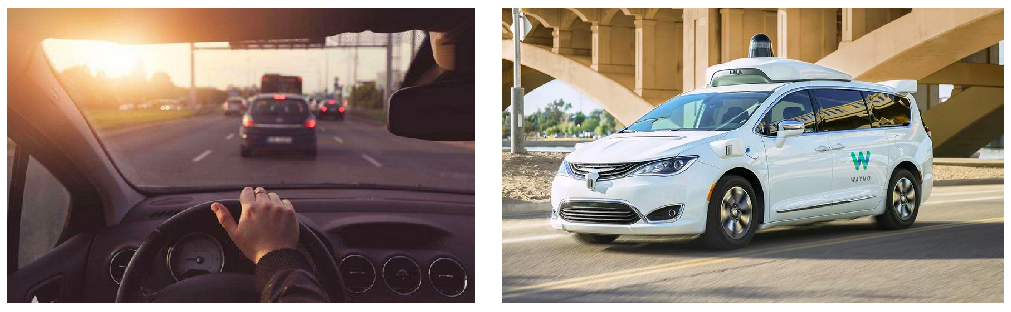
\includegraphics[width=\textwidth]{introduction/human-auto}
	\caption{Cars driven by humans versus cars driven autonomously. Humans can drive solely based on vision, while autonomous vehicles currently rely on high-precision ranging devices and backend high-precision map services.}
	\label{fig:human-auto}
\end{figure}

If we were to draw a comparison between birds and airplanes, our human driving abilities would resemble the effortless and natural flight of birds in the sky. However, for aircraft designers, should they make airplanes flap their wings like birds? The reality is quite different. Aircraft possess sophisticated control devices to manipulate airflow over their wings to generate the necessary lift; they also have precise measuring instruments to determine their own attitude and use modern control methods to maintain the desired orientation. The relationship between autonomous and human-driven vehicles is very similar to that of airplanes and birds. We can draw upon certain human abilities to design autonomous driving systems, but the resulting autonomous vehicles will inevitably differ significantly from human-driven ones. We don't necessarily need autonomous vehicles to behave exactly like human-driven ones. Autonomous vehicles should have their own design and operational logic.

In fact, autonomous driving vehicles are already capable of providing automated driving experiences. In several major cities in China (such as Beijing, Shanghai, Changsha, Chongqing, Wuhan, Shenzhen, among others), autonomous taxis (Robotaxis) has been opened to the public and can be experienced at any time. If you were to sit in an autonomous vehicle, you would notice that the steering wheel turns automatically, and braking and acceleration do not require human intervention. You might realize that if the vehicle were entirely controlled by a computer, there would be no need to install those steering wheels, pedals, or central control panels in the car. Additionally, you can see on the vehicle screen the planned route, surrounding vehicles and pedestrians, and data provided by HD maps. Since 2018, these vehicles have undergone several years of pilot testing but have not yet reached mainstream consumers.

On the other hand, if you were looking to buy a vehicle soon, most vehicles would advertise their autonomous driving features. They can automatically maintain a fixed speed on highways, eliminating the need for you to operate the accelerator; they can also automatically steer to keep the vehicle in the center of the lane, relieving you of steering duties. Some vehicles even offer features like lane change assistance or automatic lane changing, so you can leave lane changing to the vehicle. They can even handle automatic following in congested traffic conditions. These features indeed assist drivers in vehicle operation. Moreover, these vehicles are tangible and can be purchased at widely accepted prices. Most of them use purely visual or predominantly visual sensor solutions.

Are all of these considered "autonomous driving"? If so, why is it difficult to purchase the former now, while the latter can appear directly on the consumer market?

This is precisely the situation that autonomous driving faces today: if we want to achieve driving capabilities similar to humans and have vehicles drive entirely on their own without the need for drivers, it requires a hefty price to implement such functionality. This cost could be attributed to laser radar sensors, backend map services, machine costs, research and development investments, and so on. When vehicles no longer require drivers, many business models will change accordingly. Taxi companies will no longer need drivers, food delivery companies will no longer need delivery personnel, and all operational personnel will only need to maintain autonomous driving vehicles. On the other hand, if we want to keep the price of vehicles within the reach of consumer-grade vehicles by using inexpensive, practical sensors, then we must acknowledge the current lack of reliability in existing algorithms, necessitating human driver supervision and intervention at any time, unable to completely replace human drivers. In fact, the entire autonomous driving industry is currently exploring along these two paths. The former path is highly likely to lead to fully autonomous driving, but currently, it seems too expensive to be directly targeted at consumers; the latter path is known as the "incremental" route, which is being used by various vehicle manufacturers, but it still has a significant distance from fully autonomous driving and is not suitable for tasks that require fully autonomous driving capabilities.

This divergence in paths reminds us that sometimes when discussing autonomous driving, different parties may not necessarily be talking about the same tasks. In fact, if we only care about "some" autonomous driving tasks, such as automatic following, lane keeping, and automatic lane changing, they do not require very complex technology or sensors. Although we sometimes refer to these vehicles as "autonomous driving" vehicles, and their manufacturers are also willing to claim that they are "fully autonomous driving," they still belong to the category of "assisted driving" functions according to standards. This also reminds us that there should be a clear and standardized delineation of autonomous driving capabilities.

In the international arena, researchers have long classified vehicles into five levels of autonomy, from Level 1 to Level 5 (SAE classification\footnote{Classification by the Society of Automotive Engineers, see SAE Standard J3016-202104: \url{https://www.sae.org/standards/content/j3016_202104}.}), as shown in \autoref{table:SAE}. Similar to this, China has its own "Classification of Automotive Driving Automation"\footnote{See: GB/T: 40429-2021.}, the summary of which is presented in \ref{table:GBT-Chinese}. Generally, the various standards for classifying autonomous driving capabilities are primarily based on the following two points:

\begin{enumerate}
\item Whether the system requires human intervention, also known as \textbf{intervention}. \textbf{Assisted driving systems} require the driver to take over when intervention is needed, while \textbf{autonomous driving systems} strive to operate without the need for human intervention, allowing the removal of driver equipments such as steering wheels and pedals. This is the key distinction between Level 2 and above Level 3 autonomous driving capabilities.
\item Whether the system operates in limited scenarios or can function in most normal scenarios relative to human drivers. This is the key difference between Level 4 and Level 5.
\end{enumerate}

\begin{table}[h]
	\footnotesize
	\caption{SAE Automated Driving Levels}
	\label{table:SAE}
	\centering
	\begin{threeparttable}
	\begin{tabular}{|c|ccc|ccc|}
		\hline Level & L0 & L1 & L2 & L3 & L4 & L5 \\\hline
		Responsiblity & \multicolumn{3}{c}{Driver} & \multicolumn{3}{c|}{Computer} \\\hline
		Intervention & \multicolumn{3}{c|}{at all times} & when required & \multicolumn{2}{|c|}{not required} \\\hline
		Typical Func. & \makecell[l]{AEB\\BSD\\ LDW \\ ALC} & \makecell[l]{LCC\\ACC} & LCC+ACC & \makecell[l]{Traffic Jam Driving\\Auto Parking\\Auto Summoning} & \makecell[c]{Robotaxi\\Robotruck} & all conditions \\\hline
	\end{tabular}
	\begin{tablenotes}
	\item Abbreviations: LDW: Lane Departure Warning, ACC: Adaptive Cruise Control, LCC: Lane Centering Control, BSD: Blind Spot Detection, AEB: Automatic Emergency Braking, ALC: Auto Lane Change.
	\end{tablenotes}
	\end{threeparttable}
\end{table}

\begin{table}[h]
	\footnotesize
	\caption{China Classification of Automotive Driving Automation}
	\label{table:GBT-Chinese}
	\centering
	\begin{tabular}{|c|c|c|}
		\hline Driving Level & Name & Main Contents \\\hline
		L0 & Emergency Assist. & \makecell[l]{Detection and response capabilities for certain events} \\
		L1 & Partial Driver Assist. & \makecell[l]{Continuous execution of lateral and longitudinal control} \\
		L2 & Combined Driver Assist. & \makecell[l]{Continuous execution of lateral and longitudinal control} \\
		L3 & Conditionally Auto. Driving & \makecell[l]{Continuous execution of all driving tasks} \\
		L4 & Highly Auto. Driving & User may refrain from taking over \\ 
		L5 & Fully Auto. Driving & Can autonomously drive in any environment \\\hline
	\end{tabular}
\end{table}

Therefore, although there are five to six levels in terms of classification, for professionals in the field of autonomous driving, the main concern lies in Levels 2 and 4. Level 2 autonomous driving vehicles can be directly targeted at consumers, enhancing driving comfort to a certain extent based on traditional vehicles. The functionalities currently achieved at Level 2 are not far from current laws and regulations and are gradually being popularized in some new car models. On the other hand, Level 4 vehicles should be capable of unmanned driving in most scenarios, able to address some business needs for automation, which is also considered by many researchers as a form of "driverless" mode. Although within the broad definition, both Level 2 and Level 4 are part of autonomous driving, in practical terms, there are fundamental differences in module design and implementation between them. Level 4 autonomous driving is most concerned with the \textbf{intervention rate}, requiring that the vehicle cannot be taken over by human without cause, thus placing high demands on various algorithm performances. On the other hand, all functions of Level 2 autonomous driving can be taken over by humans, thus emphasizing the recognition of which scenarios are \textbf{valid scenarios}, where Level 2 functionalities can be activated. Due to human intervention, Level 2 is much more tolerant of most algorithm metrics, placing greater emphasis on the presence of functions rather than complete automation.


\begin{figure}[!htp]
	\centering
	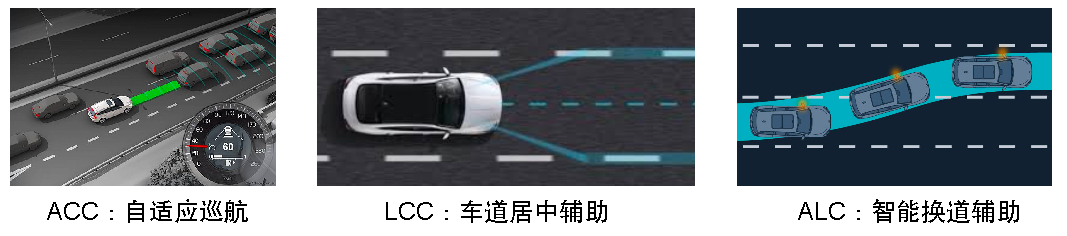
\includegraphics[width=1.0\textwidth]{introduction/l2-tasks}
	\caption{Typical L2 tasks: ACC, LCC, ALC. }
	\label{fig:l2-tasks}
\end{figure}

\subsection{Typical L4 Tasks}
L2 or L4, that is the question.

However, this question shouldn't be answered by technical personnel. We should first ask, does a certain type of vehicle really need to drive completely autonomously? In some scenarios, the answer is ``yes''. \textbf{Automation} is the core functionality of these vehicles. Without full automation, these vehicles lose their raison d'être. In other scenarios, we might say ``not necessarily.'' What we need more is safe driving with computers helping to \textbf{alleviate burdens}. If computers can provide more advanced functions, we are willing to accept them, but we also need to consider the cost of these functions. If the cost is too high, consumers won't buy it.

\begin{figure}[!t]
	\centering
	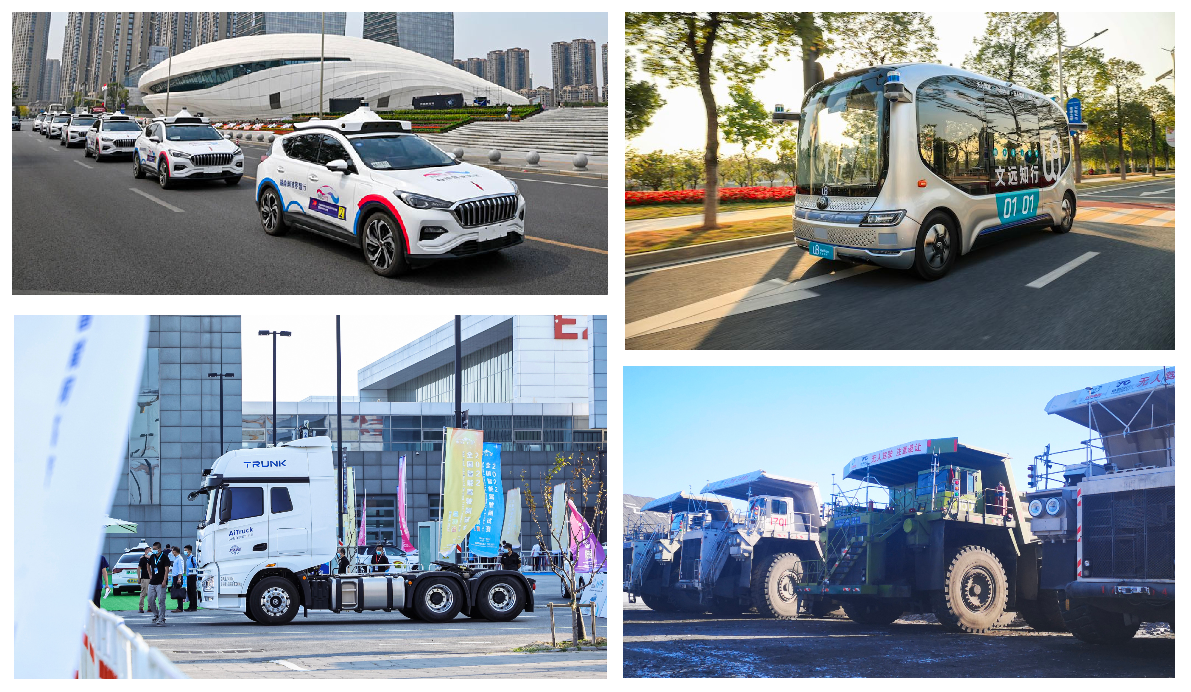
\includegraphics[width=1.0\textwidth]{introduction/l4-robotaxi}
	\caption{Some applications of L4 passenger vehicles: autonomous taxis, buses, trucks, mining trucks}
	\label{fig:l4-robotaxi}
\end{figure}

The former belongs to typical L4 applications, and the entity doesn't have to be limited to \textbf{vehicles}. In a broad sense, as long as a chassis carries sensors and has a certain level of automation, it can be considered a form of autonomous driving vehicle. From this perspective, whether the entity is a car or carries passengers is not the key to distinguishing autonomous driving. Whether the tasks they perform require \textbf{full automation} is the key to distinguishing their autonomous driving capabilities. For example, an autonomous delivery vehicle's primary function is to autonomously deliver items to users. If this function isn't fully automated and still requires a driver's cooperation, then the business loses its main feature. An autonomous cleaning vehicle's main function is to automatically cover cleaning in fixed scenes. If this process still requires human involvement, it's not meaningful. For these businesses, \textbf{removing the driver} is their most important feature, so they belong to core L4 applications. These vehicles are not designed with driver cabins or driver positions (Figure~\ref{fig:l4-lowspeed}).


\begin{figure}[!t]
	\centering
	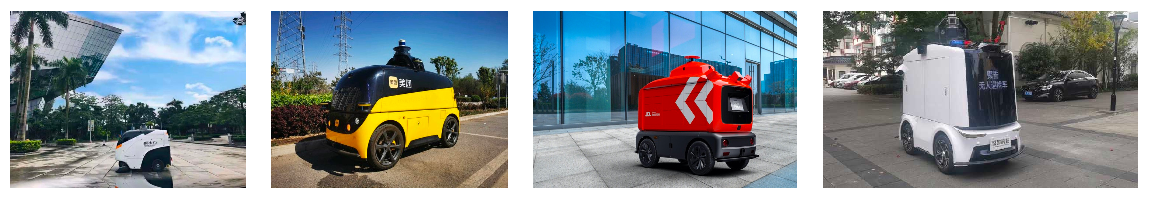
\includegraphics[width=1.0\textwidth]{introduction/l4-lowspeed}
	\caption{Low-speed L4 applications: sweepers, delivery bots, patrol robot}
	\label{fig:l4-lowspeed}
\end{figure}

On the other hand, we can also ask, do taxis need autonomous driving? Do trucks need autonomous driving? If there are no drivers, taxis can be operated solely by taxi companies, and trucks can also be operated solely by logistics companies, without the need to recruit drivers, only requiring vehicle maintenance. This business model is called Robotaxi and Robotruck, which is a completely different way from existing commercial models (see Figure~\ref{fig:l4-robotaxi}). It imposes strict requirements on autonomous driving. Once a vehicle experiences a failure and requires human intervention, in the absence of a driver on board, it's difficult to have a human driver intervene in a timely manner, and a takeover event could easily turn into an accident.

Applications such as Robotaxi, Robotruck, Robobus, etc., technically also belong to L4 autonomous driving. Compared to autonomous driving vehicles for cleaning, delivery, inspection, etc., they have higher requirements for autonomous driving safety, stricter requirements for overall vehicle system stability, lower tolerance for risks and failures, and require more perception, high-precision positioning, mapping, and other technical support. If a low-speed vehicle experiences a failure, it won't directly lead to casualties, and most of the time, it can be remotely managed by technical personnel. However, if a passenger-carrying vehicle experiences an accident, the consequences can easily have substantial impacts at the company or even the community level. So, we ask, can the current level of technology support applications like Robotaxi? Unfortunately, this question currently does not have a definitive answer.

On one hand, autonomous driving systems are complex systems, unlike traditional electronic or mechanical switches, where it's easy to provide a functional safety verification plan or give clear reasons for failures. If an autonomous driving vehicle fails to recognize a vehicle in front and collides, within the current theoretical framework, we can't explain \textbf{why the system failed to recognize the vehicle ahead}. It's just a phenomenon that occurs in reality. Perhaps if a certain value in a certain program is increased by 0.001, this phenomenon won't occur, but it may make it impossible to recognize vehicles of a different color in different weather conditions. There are hundreds of millions of parameters like this, none of them have names, and they are connected and calculated in a way arbitrarily stipulated by humans. It's difficult to attribute the occurrence of a specific result to a parameter being too large or too small, or the calculation sequence between them not being reasonable enough. A brake system is almost impossible to fail, but a perception system is almost impossible to be 100\% correct. In short, autonomous driving systems are difficult to precisely analyze what failure at a certain point may lead to what phenomenon, and provide convincing reasons, like traditional mechanical and electronic systems.

On the other hand, if it's difficult to verify the safety of autonomous driving vehicles from a theoretical level, can we statistically measure the stability of autonomous driving systems at an experimental level? This is indeed what many autonomous driving companies are doing now. Most L4 autonomous driving companies will statistically analyze the relationship between vehicle mileage and takeover times, for example, calculating the \textbf{miles per intervention} (MPI)\footnote{Sometimes also called miles per disengagement, MPD.}, to measure the stability of the system. In the 2021 report of the California Department of Motor Vehicles (DMV) on autonomous driving, the MPI of some Chinese companies has reached the level of thousands to tens of thousands of kilometers (see Table~\ref{table:l4-mpi})\footnote{Source: \url{http://www.evinchina.com/articleshow-217.html}}. We generally believe that MPI is indeed an indicator of the overall autonomous driving capability of a vehicle, but so far, there is no very open and fair MPI testing method, and what we can see more are self-testing reports from various companies. They lack unified testing environments and standardized criteria for when to intervene. In terms of quantity and mileage, compared to traditional mass-produced vehicles, most L4 autonomous driving companies only have fleets consisting of dozens or hundreds of vehicles, and their road test scenarios are usually relatively simple. Compared to traditional manufacturers with monthly sales of tens of thousands of vehicles, their accumulated test mileage and number of scenarios are very limited.

%\begin{figure}[!t]
%	\centering
%	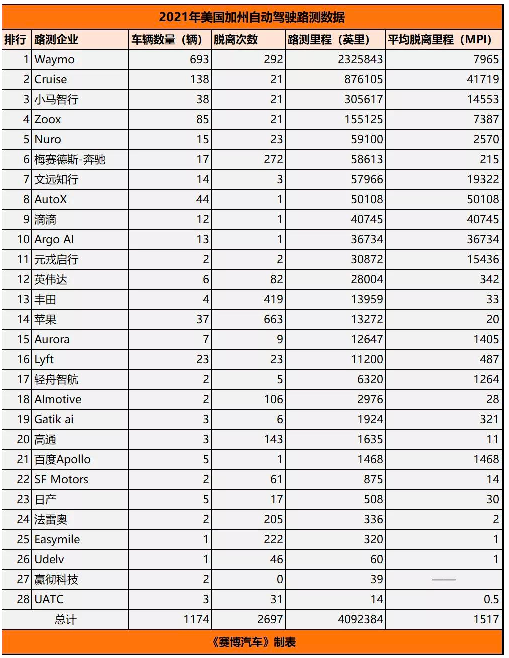
\includegraphics[width=0.7\textwidth]{introduction/l4-mpi}
%	\caption{2021 report of the California Department of Motor Vehicles (DMV) on autonomous driving}
%	\label{fig:l4-mpi}
%\end{figure}

\begin{table}[!t]
	\footnotesize
	\caption{2021 report of the California Department of Motor Vehicles (DMV) on autonomous driving}
	\label{table:l4-mpi}
	\centering
	\begin{tabular}{c|llll}
		\hline\hline Company & Num. of cars & Num. of Invent. & Miles & MPI \\\hline
		Waymo & 693 & 292 & 2325843 & 7965 \\\hline
		Cruise & 138 & 21 & 876105 & 41719 \\\hline 
		Pony.ai & 38 & 21 & 305617 & 14553 \\\hline
		Zoox & 85 & 21 & 155125 & 7387 \\\hline 
		Nuro & 15 & 23 & 59100 & 2570 \\\hline
		Mercedes-Benz & 17 & 272 & 58613 & 215 \\\hline 
		WeRide & 14 & 3 & 57966 & 19322 \\\hline 
		AutoX & 44 & 1 & 50108 & 50108 \\\hline
		DiDi & 12 & 1 & 40745 & 40745 \\\hline 
		Argo AI & 13 & 1 & 36734 & 36734 \\\hline 
		DeepRoute.ai & 2 & 2 & 30872 & 15436 \\\hline 
		Nvidia & 6 & 82 & 28004 & 342 \\\hline 
		Toyota & 4 & 419 & 13959 & 33 \\\hline
		Apple & 37 & 663 & 13272 & 20 \\\hline 
		Aurora & 7 & 9 & 12647 & 1405 \\\hline 
		Lyft & 23 & 23 & 11200 & 487 \\\hline 
		Almotive & 2 &106 & 2976 & 28 \\\hline 
		Gatik ai & 3 & 6 & 1924 & 321 \\\hline 
		Qualcomm & 3 & 143 & 1635 & 11 \\\hline 
		Apollo & 5 & 1 & 1468 & 1468 \\\hline 
		SF Motors & 2 & 61 & 875 & 14 \\\hline 
		Nissan & 5 & 17 & 508 & 39 \\\hline 
		Valeo & 2 & 205 & 336 & 2 \\\hline 
		Easymile & 1 & 222 & 320 & 1 \\\hline
		Udelv & 1 & 46 & 60 & 1 \\\hline
		Inceptio.ai & 2 & 0 & 39 & - \\\hline 
		UATC & 3 & 31 & 14 & 0.5 \\\hline\hline
	\end{tabular}
\end{table}

The dilemma of whether to have vehicles first or autonomous driving technology first is facing all L4 autonomous driving companies. Without a sufficient number of vehicles, it's difficult to prove that an autonomous driving system is stable enough, and thus challenging to truly implement businesses like Robotaxi; however, if we focus solely on the vehicle itself without paying attention to autonomous driving technology, it's also challenging to attract enough technical talents and cultivate the team's technical capabilities. Several years ago, it was a common problem that L4 technology companies didn't understand vehicles, and vehicle manufacturers didn't understand autonomous driving. Doing both requires enormous scale and determination, while collaboration between two different companies requires a high level of trust. Fortunately, major vehicle manufacturers have begun to pay attention to autonomous driving-related businesses (although currently focused on the easier-to-implement L2 business), and L2-related functionalities have been integrated into many vehicle models. Many practitioners also believe that as autonomous driving technology matures, L2 functionalities will gradually become richer and gradually approach L4 capabilities. Suppliers of autonomous driving-related sensors, algorithms, chips, and hardware will also play active roles in various vehicle models.

Even after overcoming technical issues, businesses like Robotaxi still face practical legal and social issues. After all, if L4 vehicles are widely deployed, other drivers will face the challenge of how to interact with driverless vehicles\footnote{Throughout this book, the term \textbf{driverless vehicles} generally refers to L4 autonomous driving vehicles.}. Will driverless vehicles understand the intentions of other vehicles changing lanes or overtaking? Will they avoid vehicles driving in the wrong direction? Will they detour around road sections undergoing sudden construction? Will they recognize children who have fallen on the road? Legally, how should the responsibility of driverless vehicles be defined if they collide with other vehicles? Should the responsibility lie with the developer of the driverless vehicle? Should the developers be held accountable if the collision occurs because the perception system failed to correctly identify pedestrians, or because the map annotation personnel incorrectly annotated the speed limit information of a road section, or because the satellite signal was weak that day, causing the vehicle to enter the wrong lane? These are questions that may be encountered in reality but are difficult to answer. In vehicles with human drivers, most safety responsibilities ultimately fall on the driver. Once the subject becomes a driverless vehicle, these responsibilities are difficult to distribute among various modules. It's unlikely that any company currently has the ability to assume these responsibilities on behalf of autonomous driving development companies. In short, discussions on many legal, ethical, and social issues related to autonomous driving will continue for many years to come.

However, autonomous driving still represents the direction of future technological advancement. Its overall prospects are promising, albeit with inevitable challenges along the way. Future passenger vehicles, low-speed vehicles, and robots will become increasingly intelligent, taking on more and more tasks in daily life. A series of technical issues derived from autonomous driving will also be fully addressed and discussed by researchers in various fields. Many things that appeared in science fiction movies will gradually become familiar landscapes in the coming years. For example, restaurant robots that the author fantasized about during their studies were once among the representatives of science fiction, but now they are widely present in major shopping malls, and major suppliers have begun price wars. Will autonomous driving vehicles also experience this situation in the coming years? We wait and see.

\section{Localization and Mapping in Autonomous Driving}
\subsection{Why L4 Needs Localization and Mapping}
This book primarily discusses the localization and mapping technologies in L4 autonomous driving. Before delving into the details, readers might ask a fundamental question: why does autonomous driving require localization and mapping?

That's an excellent question. My answer is, if high-precision localization and mapping weren't necessary for autonomous driving, that would be ideal. Unfortunately, at the current technological level, achieving low intervention rates in L4 autonomous driving still requires the use of high-precision localization and mapping. Conversely, if we're discussing L2 autonomous driving, which doesn't prioritize intervention rates, high-precision localization and mapping may not be necessary (although some L2 systems are also using high-precision maps) \cite{Zhang2021, Ort2020, Can2020}. This contradicts the current level of intelligence and reliability. The smarter it is, the less reliable it becomes; the more reliable it is, typically meaning simpler in structure, the less intelligent it is. If we choose to accept the results of AI, we must also accept the mistakes made by AI. As for when L4 is needed and when L2 is needed, we've discussed this earlier.

\begin{figure}[!t]
	\centering
	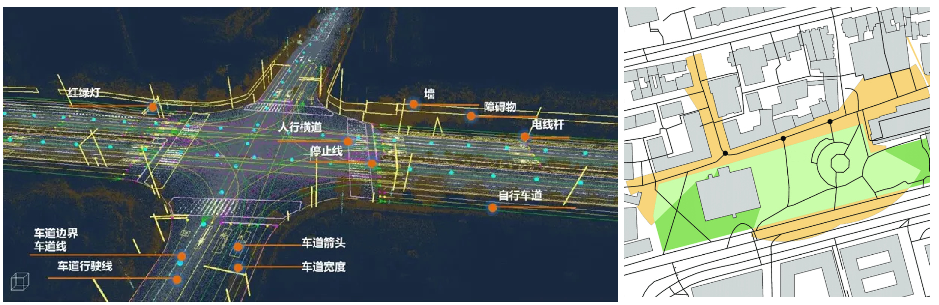
\includegraphics[width=1.0\textwidth]{introduction/hdmap}
	\caption{Differences between high-definition maps and traditional electronic navigation maps. Navigation maps represent roads and intersections using polygons and vectors, while high-definition maps also accurately mark lane positions, stop line positions, and provide detailed information about surrounding objects.}
	\label{fig:hdmap}
\end{figure}

Why does L4 need high-definition maps? This is because L4 and L2 have different goals. L2 autonomous driving doesn't concern itself with intervention rates, whereas achieving low intervention rates is the primary goal of L4, which determines that their technological paths have fundamental differences. L4-related technologies exhibit strong determinism. Many behaviors that may seem acceptable at the L2 level, such as turning into the wrong lane at an intersection or misreading a traffic light, would result in intervention in L4 and are not allowed to occur. Consequently, L2 leans more toward real-time perception and may even use perception results directly to construct a bird's eye view (BEV) \cite{Sun2020, Ng2020, Hendy2020}, while L4 relies on offline maps \cite{Levinson2010, Wolcott2014, Matthaei2014}. In simple terms, L2 is more like ``driving while looking at the road,'' whereas L4 is ``driving in the map in the mind.'' ``Driving while looking at the road'' has the advantage of very direct logical relationships, closer to human behavior, but the disadvantage is dealing with the limitations and uncertainties of computer detection results. Vehicle cameras typically only see the ground lane lines a few dozen meters ahead. They may also be obscured by other vehicles, submerged in puddles, or, due to lighting conditions, shadows of roadside guardrails may be mistaken for lane lines. These outcomes could affect the vehicle's autonomous driving behavior, and these uncertainties must be considered at the control and decision-making levels. In contrast, high-definition maps in L4 are meticulously annotated by humans, with accurate positions for each lane. It's predetermined which lane they will continue onto, which direction to turn at intersections, and which traffic light to look at in three-dimensional space \cite{Ghallabi2018}. Even if no lane lines are visible in real-time images, L4 vehicles can accurately follow straight lines in the map \cite{Yang2018}. This approach comes with two costs: first, we need to create such a high-definition map in advance; second, we need to know our accurate position in this map \cite{Spangenberg2016, Levinson2007}.

High-precision localization and mapping represent a strict, accurate concept. On the flip side, it brings about rigid, cumbersome business burdens. Maps essentially transform those limited, uncertain perception elements into static, precise data information through manual or post-processing methods (Figure \ref{fig:hdmap}). Maps carry out similar tasks to real-time perception but can provide correct results across unlimited ranges, greatly reducing the burden of perception \cite{Seif2016}. Therefore, some have said that maps are a cheating sensor, essentially providing the answers directly to autonomous driving vehicles. With high-definition maps, the vehicle's burden of perception can be significantly alleviated. We only need to focus on dynamic pedestrian and vehicle information, without worrying about the shape and topology of road lanes. However, the balance between maps and perception is constantly changing. Some companies' high-definition maps are richer than others, even including information about obstacles, flowerbed shapes, etc., while others' solutions require the perception module to detect this information. Perhaps in the near future, the balance between maps and perception will change with technological iterations.

In current L4 autonomous driving solutions, most task elements are tied to maps. When users want to drive from point A to point B in a city, the autonomous driving vehicle first generates a lane-level path from point A to point B on the map. This path is different from the common navigation systems we're familiar with; it's at the lane level. The navigation system calculates which road, which intersection, and which lane to turn into. When executing autonomous driving tasks, the vehicle also strives to ensure that the actual executed path aligns with the results of high-definition map navigation. For this reason, the vehicle needs to know its real-time position on the map, which requires high-precision localization within lanes.

\subsection{Contents and Production of High-Definition Maps}

High-definition maps are essentially \textbf{structured data} \cite{Zhou2021}. Their basic elements consist of sections of lanes in the real world, as depicted in Figure \ref{fig:hdmap-lane}. Various questions about lanes can be asked, such as:
\begin{enumerate}
	\item What is the geometric shape of this lane? Is it straight, with bends, or curved?
	\item Which lane is to its left, and which is to its right?
	\item What is the speed limit? Is it a straight lane or a turning lane?
	\item Is it a motorized lane or a non-motorized lane?
	\item Which lanes is it connected to? Are they sequentially connected, or are there forks or mergers?
\end{enumerate}

\begin{figure}[!t]
	\centering
	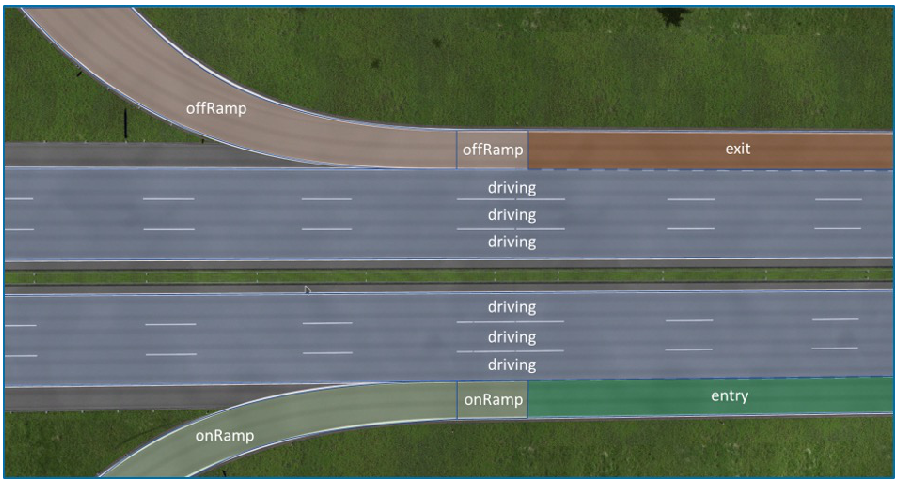
\includegraphics[width=0.7\textwidth]{introduction/hdmap-lane}
	\caption{Common lane information in high-definition maps}
	\label{fig:hdmap-lane}
\end{figure}

\begin{figure}[!t]
	\centering
	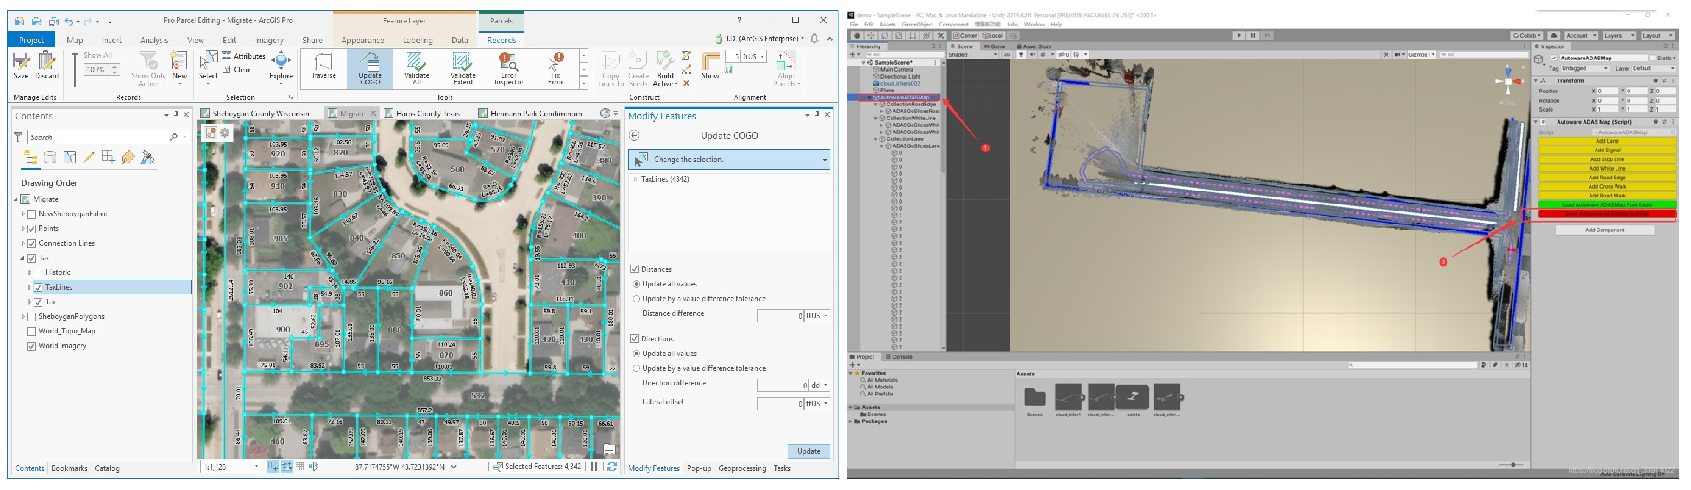
\includegraphics[width=1.0\textwidth]{introduction/hdmap-editor}
	\caption{Common high-definition map editing software: ArcGIS and Autoware Map Tool}
	\label{fig:hdmap-editor}
\end{figure}

Questions of this sort are easily described and stored using \textbf{structures} in programs. Various programming and markup languages support struct syntax, making high-definition map software compatible with multiple languages, including JSON, Protocol Buffers (protobuf), XML, and others. Describing a complete lane's information can be quite extensive and challenging. Researchers worldwide have therefore developed standards for high-definition maps. Common standards include OpenDrive \cite{Dupuis2010}, LaneLet2 \cite{Poggenhans2018}, and Apollo OpenDrive. These standards define ways to describe a lane, an intersection, and specifics of various traffic lights. Readers can refer to these standards for a comprehensive understanding of field information.

Most geometric elements in high-definition maps are described by points. For instance, a lane can be described by its center reference line plus its width, or by lines marking its left and right boundaries, which are composed of a series of lower-level points. The coordinates of each point can be expressed in terms of latitude and longitude or other global coordinate systems discussed later. Typically, they are represented by floating-point numbers. On the other hand, area-like elements can be described by polygons formed by multiple points, such as parking lots or buildings. Once this information is exported to files, it can be used for map rendering or for vehicle navigation and control.

Since high-definition maps are essentially made up of these lines and information, can't we generate them freely? Certainly, we can. We can even draw a road on paper and say its speed limit is 60 kilometers per hour; this can be considered a high-definition map, albeit with limited practical use. High-definition maps on computers are usually generated using specialized drawing software (such as ArcGIS, Autoware Map Tool, as seen in Figure \ref{fig:hdmap-editor}), and some companies may develop their own drawing software. You can certainly start from a blank area and draw a virtual map. However, if we want the map to correspond to the real world, we need to find a way to first obtain the three-dimensional structure or two-dimensional aerial view of the real world. These serve as the data source for real-world high-definition maps.

\begin{figure}[!t]
	\centering
	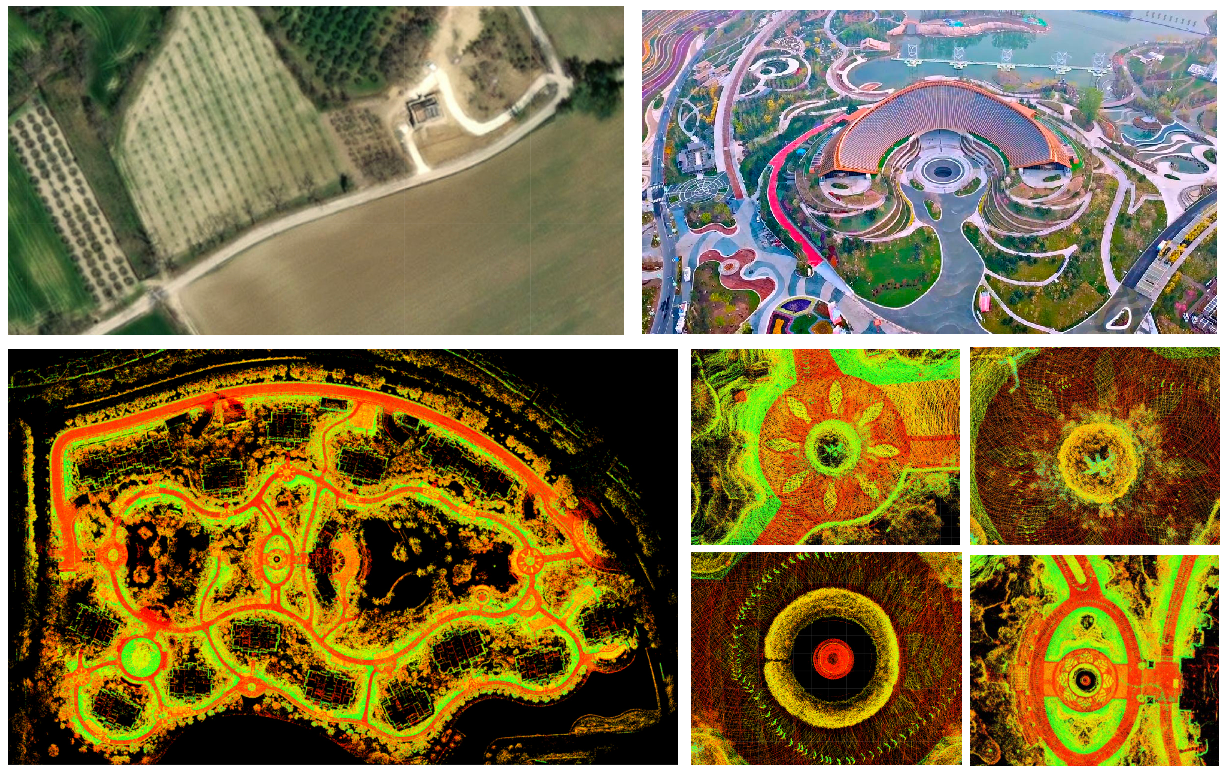
\includegraphics[width=1.0\textwidth]{introduction/hdmap-source-image}
	\caption{Data sources for high-definition maps: satellite imagery, drone aerial imagery, laser-generated point cloud maps (global and local)}
	\label{fig:hdmap-source}
\end{figure}

The two-dimensional or three-dimensional data from the real world mainly come from the following sources:

\begin{enumerate}
	\item Satellite imagery from remote sensing satellites. Satellite imagery can be obtained in various mapping software, but the highest resolution of civilian satellite imagery is at the level of a few meters, and images become blurred at around 10 meters. While they cover the entire globe and can be used for annotating electronic navigation maps, they are insufficient for high-definition maps, making it difficult to discern the specific positions of lanes and road surface details (see Figure \ref{fig:hdmap-source}, top left).
	\item Aerial imagery from drones. Drones equipped with high-precision positioning devices can take top-down photographs at any altitude, which are then stitched together to create aerial imagery. This imagery can be highly detailed, but its coverage is limited, and flying drones is prohibited in many areas.
	\item Three-dimensional map reconstruction using sensors carried by autonomous vehicles. The most common method is to use onboard LiDAR sensors to construct three-dimensional point clouds of the scene. These point clouds reflect the three-dimensional structure and brightness information of the scene and can effectively serve as a reference for map drawing. Since autonomous vehicles have relatively unrestricted ranges of travel, most autonomous driving companies use this method to construct point cloud maps \cite{Ghallabi2019, Ma2019}.
\end{enumerate}

Figure \ref{fig:hdmap-source} shows several different data sources. They follow a simple logic: the closer they are, the clearer they appear. Compared to remote sensing satellites orbiting tens of thousands of kilometers above the Earth, drones can hover tens of meters above the ground, while cars can directly capture images or measure distances in front of objects. Satellite images often struggle to discern road surface details, while drone images and LiDAR point clouds can reflect the texture of the road, the shapes of tree trunks and trees, and various small objects in the scene. Based on vehicle point clouds, we can annotate various detailed objects. If time permits, we can even annotate details such as the texture of tiles and the positions of tree trunks in high-definition maps.

\section{Introduction to SLAM in this Book}

The next question is how to use sensors onboard vehicles for high-precision point cloud reconstruction? What principles underlie this type of three-dimensional reconstruction? Apart from annotating maps, what other purposes do they serve? We will explore all of these questions throughout the content of this book. We will see that high-precision point clouds are the result of the combined action of a series of sensors. Their prices range from hundreds to hundreds of thousands, each serving different purposes. The core of the three-dimensional reconstruction system lies in estimating the vehicle's position and attitude at each moment, involving the vehicle's own \textbf{kinematic theory} and the \textbf{state estimation theory} used to estimate the vehicle's state using sensors. The following chapters of this book will introduce various sensor principles and methods in a certain order. The rough sequence is as follows:

\begin{enumerate}
	\item Firstly, we need to introduce some basic geometric knowledge, including the sensor coordinate systems on the vehicle and the coordinate systems of the Earth. At the same time, we will review the basic knowledge of state estimation theory, including the Kalman filter and nonlinear optimization theory. This part of the knowledge has been introduced in my previous book \cite{Gao2017}, so we will not elaborate further but only review. In particular, this book will mainly use properties on $\mathrm{SO}(3)$ when dealing with rotation variables. Readers need to maintain a certain proficiency in this part of the content. This is the content of Chapter 2 of this book.
	\item Chapters 3 and 4 will introduce two mainstream methods for processing \textbf{inertial measurement unit} (IMU) data. Chapter 3 introduces the classical Error State Kalman Filter (ESKF) and handles rotations in $\mathrm{SO}(3)$, while Chapter 4 mainly introduces preintegration methods. Since IMUs do not directly measure the physical state of the vehicle (translation and rotation) but rather measure their derivatives along the time axis (angular velocity and acceleration), we must introduce the differential relationship of the vehicle state and their various properties after integration. These are the main contents of Chapters 3 and 4.
	\item Chapters 5 to 7 introduce the content of laser SLAM. Chapter 5 mainly covers basic point cloud processing methods, including how to represent laser point clouds, how to find their nearest neighbors, and how to rasterize them. We will implement some classical data structures ourselves. Chapters 6 and 7 respectively introduce 2D and 3D laser SLAM methods. We will first implement some laser registration methods: 2D and 3D ICP, NDT, probability grid, etc., then manage them using sub-map methods, and finally add loop detection to form a complete SLAM system. Chapter 7 also introduces loosely coupled laser-inertial odometry.
	\item Chapters 8 to 10 introduce typical SLAM applications. Chapter 8 implements a tightly coupled laser-inertial odometry, each using an iterative error Kalman filter and a preintegration optimizer. Chapter 9 introduces offline point cloud map construction methods. We will rewrite some key algorithms into easily parallelized offline programs. Chapter 10 introduces methods for high-precision localization in existing point cloud maps. We will divide the point cloud map into small blocks in space and then use filters to achieve fusion localization of point clouds and inertial data.
\end{enumerate}

The above is the main content of this book. We mainly focus on the application of SLAM in autonomous driving around the aspects of inertial navigation and laser point clouds. Most vehicles on open roads or park roads can be mapped and located in this way. However, this book will not delve into the annotation part of maps in detail because they are mainly drawn manually and do not involve much algorithmic content\footnote{The automatic generation of high-definition maps is also a key research direction in the field of autonomous driving, but the methods are quite different from the content covered in this book, and the results are not yet mature. We will not delve into this topic. Readers can refer to related literature, such as \cite{Elhousni2020, Liao2022}.}.

Except for this chapter, the end of each chapter will include a certain number of exercises. Readers should allocate time for exercises according to their own learning progress.

% 2. math basics 
% !Mode:: "TeX:UTF-8"
\thispagestyle{empty}

\chapter{Review of Basic Mathematical Concepts}
\label{sec:math-basics}
\thispagestyle{empty}

Before delving into various sensor processing methods, let's review some fundamental mathematical concepts. This book largely follows the notation conventions established in ``Introduction to Visual SLAM''\cite{Gao2017}. To avoid redundancy, we must assume that readers are already familiar with the basic geometric knowledge presented in that book. This book does not elaborate on processes such as quaternion-to-rotation-matrix transformations in detail; instead, it briefly mentions their conclusions for readers to refer back to at any time. For topics not extensively covered in \cite{Gao2017}, this chapter provides additional explanations and derivations as appropriate.

\newpage
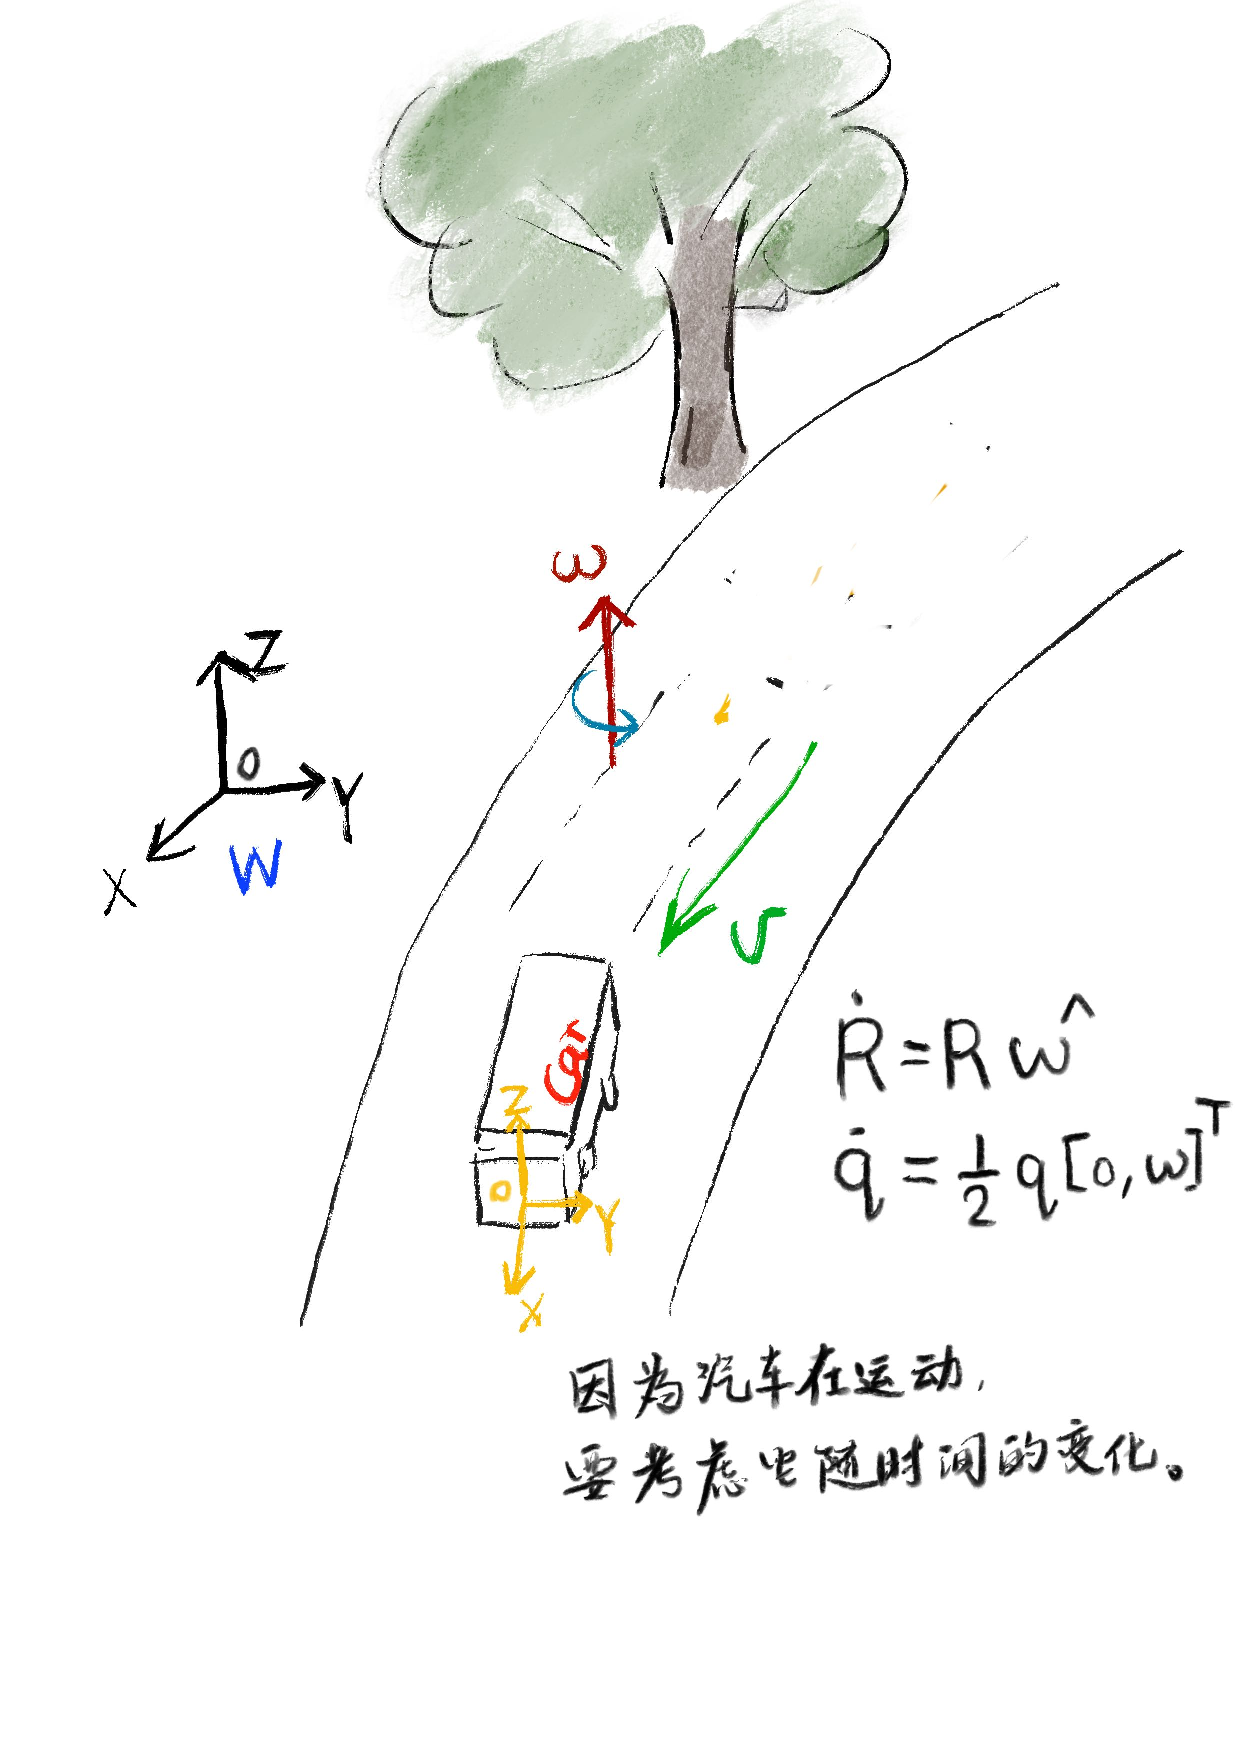
\includepdf[width=\textwidth]{art/ch2.pdf}

%\pagestyle{main}
\section{Geometry}
\subsection{Coordinate Systems}

To describe the position and orientation of an autonomous vehicle, we should first define various coordinate systems for it. Firstly, we assume the existence of a fixed coordinate system in the world, known as the \textbf{world coordinate system} or \textbf{inertial coordinate system}. There are several ways to define this coordinate system in the real world, but in principle, it can be simply considered as a fixed coordinate system. When the vehicle moves in the world coordinate system, there exists a transformation relationship between the vehicle's own coordinate system (referred to as the \textbf{body coordinate system} or \textbf{body frame}) and the world system. This transformation relationship changes over time, allowing us to define the vehicle's \textbf{linear velocity}, \textbf{angular velocity}, \textbf{acceleration}, and other physical quantities. This constitutes the motion process of the vehicle.

However, explaining what linear velocity, angular velocity, and especially attitude mean from a mathematical perspective is not so intuitive. The attitude of the vehicle is usually described by a \textbf{rotation matrix} or \textbf{quaternion}. When they change over time, how many-dimensional vectors should be used to describe the angular velocity? How does the angular velocity vector act on the rotation matrix or quaternion? Are there any formal differences in their various definitions? Are they essentially the same? These are the questions this chapter aims to answer.

A three-dimensional coordinate system is composed of three vectors in space. Typically, we choose a set of unit orthogonal vectors to form a reference frame. For instance, if $(\mathbf{e}_1, \mathbf{e}_2, \mathbf{e}_3)$ are the three vectors of the world coordinate system, it means that these three vectors have a length of 1 and their inner products are 0. In this case, we say that a coordinate system (reference frame) $E={\mathbf{e}_1, \mathbf{e}_2, \mathbf{e}_3}$ has been chosen. Then, any three-dimensional spatial vector $\mathbf{a}$ can be represented in this reference frame as:
\begin{equation}
	\mathbf{a} = a_1 \mathbf{e}_1 + a_2 \mathbf{e}_2 + a_3\mathbf{e}_3,
\end{equation}
where $(a_1, a_2, a_3)$ are the coordinates of the vector $\mathbf{a}$.

Please note that even without specifying a reference frame and coordinates, various operations can be performed between vectors. For example, the following operations can be performed between two vectors $\mathbf{a}$ and $\mathbf{b}$:

\begin{enumerate}
	\item \textbf{Addition and subtraction}. The result of vector addition or subtraction is still a vector, following the parallelogram rule:
	\begin{equation}
		\mathbf{c} = \mathbf{a} \pm \mathbf{b}.
	\end{equation}
	If the vectors have coordinates, the components are simply added or subtracted.
	
	\item \textbf{Scalar multiplication}. Multiplying a vector by any scalar $k\in \mathbb{R}$ scales the vector:
	\begin{equation}
		\mathbf{b} = k \mathbf{a},
	\end{equation}
	resulting in another vector. When $\mathbf{a}$ has coordinates, these coordinates are scaled accordingly.
	
	\item \textbf{Taking the length}. We can compute the length of a vector, denoted as:
	\begin{equation}
		\| \mathbf{a} \|.
	\end{equation}
	The length yields a scalar value. Mathematically, a vector's length can be zero or negative, for instance, in Minkowski space, but in the physical world of autonomous driving, we are concerned with vectors in Euclidean space, where their length is always non-negative.
	
	\item \textbf{Dot product}. The dot product of two vectors yields the product of their lengths times the cosine of the angle between them, resulting in a scalar:
	\begin{equation}
		\mathbf{a} \cdot \mathbf{b} = \|\mathbf{a} \| \|\mathbf{b} \| \cos \left\langle\mathbf{a},\mathbf{b} \right\rangle,
	\end{equation}
	where if vectors have coordinates, the dot product results from the sum of the products of their respective components.
	
	\item \textbf{Cross product}. The cross product of two vectors is another vector whose direction is perpendicular to the plane formed by the two vectors, and its magnitude is the product of their lengths times the sine of the angle between them. If vectors $\mathbf{a},\mathbf{b}$ are defined in the $\mathbf{e}_1, \mathbf{e}_2, \mathbf{e}_3$ frame, the cross product is written as:
	\begin{equation}
		\mathbf{a} \times \mathbf{b} = \left\| {\begin{array}{*{20}{c}}
				\mathbf{e}_1 & \mathbf{e}_2 & \mathbf{e}_3 \\
				{{a_1}}&{{a_2}}&{{a_3}}\\
				{{b_1}}&{{b_2}}&{{b_3}}
		\end{array}} \right\| = \left[ \begin{array}{l}
			{a_2}{b_3} - {a_3}{b_2}\\
			{a_3}{b_1} - {a_1}{b_3}\\
			{a_1}{b_2} - {a_2}{b_1}
		\end{array} \right] = \left[ {\begin{array}{*{20}{c}}
				0&{ - {a_3}}&{{a_2}}\\
				{{a_3}}&0&{ - {a_1}}\\
				{ - {a_2}}&{{a_1}}&0
		\end{array}} \right] \mathbf{b} \buildrel \Delta \over = { \mathbf{a}^ \wedge } \mathbf{b}.
	\end{equation}
	
	The cross product can also be expressed as the usual matrix-vector multiplication, which requires expressing the first vector in a \textbf{skew-symmetric} matrix form\footnote{A skew-symmetric matrix satisfies $\mathbf{A}^\top = -\mathbf{A}$.}. We use the $^\wedge$ symbol to define this transformation:
	\begin{equation}
		\mathbf{a}^\wedge = \left[ {\begin{array}{*{20}{c}}
				0&{ - {a_3}}&{{a_2}}\\
				{{a_3}}&0&{ - {a_1}}\\
				{ - {a_2}}&{{a_1}}&0
		\end{array}} \right] = \mathbf{A}.
	\end{equation}
		
	Note that this operator is a \textbf{one-one mapping}, meaning that for any vector, there exists a unique corresponding skew-symmetric matrix, and vice versa. We use the $^\vee$ symbol to denote the mapping from skew-symmetric matrix to vector:
	\begin{equation}
		\mathbf{A}^\vee = \mathbf{a}.
	\end{equation}
	
	The skew-symmetric matrix operator is a symbol widely used in the subsequent text; readers should pay attention to this notation. In other literature, it might also be denoted as $\mathbf{a}_\times, \mathbf{a}^\times, [\mathbf{a}]_\times, \hat{\mathbf{a}}$\cite{Qin2018}, all of which have the same meaning. This book uniformly adopts the $\wedge$ and $\vee$ symbols on the upper right, as they appear more concise.
\end{enumerate}
	
Lastly, even when a reference frame is not specified, vectors can undergo the aforementioned operations. Their results are independent of the choice of reference frame. If a reference frame and coordinates are specified, then the aforementioned computations can also be represented using numerical values of coordinates.

\begin{figure}[!htp]
	\centering
	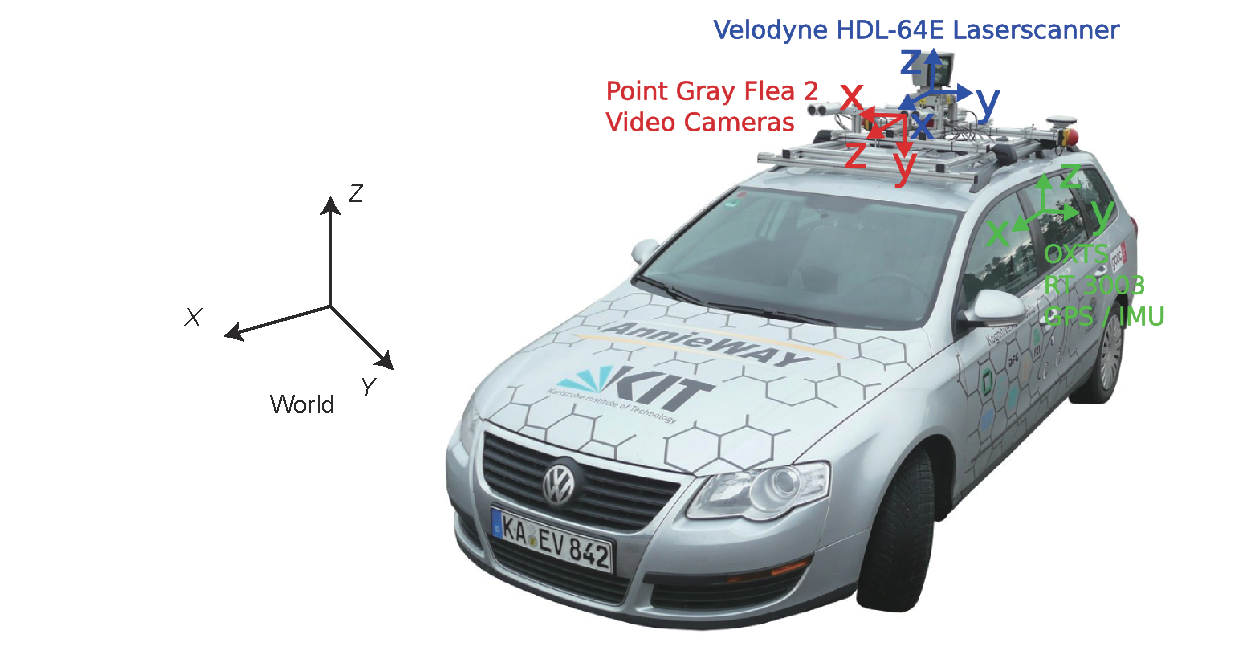
\includegraphics[width=0.7\textwidth]{math-basics/coordinate-system.pdf}
	\caption{The body and world coordinate systems of a typical autonomous vehicle sensors}
	\label{fig:corrdinate-system}
\end{figure}

An autonomous vehicle is equipped with various types of sensors. We typically assume that each sensor has its own reference frame, and their respective axis directions are defined according to the usage habits of each sensor. For example, in Figure~\ref{fig:corrdinate-system}, the IMU, 64-line lidar, and camera of the vehicle all define their own reference frames. The vehicle body generally uses the \textbf{front-left-up}\footnote{The convention "front-left-up" refers to the $X$ axis pointing forward, the $Y$ axis pointing left, and the $Z$ axis pointing up, following the right-hand rule. The convention for "right-front-up" is analogous.} or \textbf{right-front-up} order to define its coordinate system, while the camera coordinate system commonly adopts the \textbf{right-down-front} order. Consequently, there exist rotation and translation relationships between the coordinate systems of various sensors, which we characterize using rotation matrices and translation vectors.

Assuming a point $\mathbf{p}$ in the world coordinate system has coordinates $\mathbf{p}_w$, and its coordinates in the vehicle body coordinate system are $\mathbf{p}_b$, then we define the rotation matrix $\mathbf{R}_{wb}$ and the translation vector $\mathbf{t}_{wb}$, such that:

\begin{equation}
	\mathbf{p}_w = \mathbf{R}_{wb} \mathbf{p}_b + \mathbf{t}_{wb},
\end{equation}

It is crucial for readers to understand the approach here. The key points are as follows:
\begin{enumerate}
	\item Firstly, we define the transformation relationship between \textbf{coordinates}. $\mathbf{R}_{wb}$ and $\mathbf{t}_{wb}$ are used to handle coordinate transformations between vectors. Some materials deal with transformations between \textbf{coordinate axes} (or bases), interpreting rotation and translation as a transformation of a \textbf{coordinate axis} from one position to another. This definition is opposite to that of this book\footnote{One deals with transformations of coordinates, while the other deals with transformations of bases. Readers should be cautious.}, so please be careful.
	\item We can directly write $\mathbf{R}_{wb}, \mathbf{t}_{wb}$ as a \textbf{transformation matrix} $\mathbf{T}_{wb}$, expressing coordinate transformations in homogeneous form:
	\begin{equation}
		\mathbf{p}_w = \mathbf{T}_{wb} \mathbf{p}_{b}.
	\end{equation}
	This transforms the discussion into properties of the transformation matrix $\mathbf{T}$. The specific form of $\mathbf{T}$ is:
	\begin{equation}
		\mathbf{T}_{wb} = \begin{bmatrix}
			\mathbf{R}_{wb} & \mathbf{t}_{wb} \\
			\mathbf{0} & 1
		\end{bmatrix} \in \mathbb{R}^{4 \times 4}.
	\end{equation}s
	However, since the subsequent discussion will involve the IMU, which does not directly measure the differential of $\mathbf{T}$, we prefer to separate $\mathbf{R}$ and $\mathbf{t}$ rather than express them in the form of a transformation matrix.
	\item Our subscript reading order is \textbf{from right to left}, meaning the subscript $wb$ is right-multiplied with $b$ to obtain variables in the $w$ system. This makes writing and reading more fluid and intuitive. Different books handle the superscript and subscript of coordinate systems differently. Some write them on the left, some write them above, and some books even have four different markings (superscript, subscript, left, right) for one variable. This book uniformly uses the subscript $wb$ to define various variables. Since all variables have the subscript $wb$, we omit these subscripts in the vast majority of content to strive for simplicity. We also need to discuss various variables at different times or iteration numbers, which will introduce subscripts related to time or iteration numbers. If combined with coordinate system subscripts, readers would have to face a large number of formulas with various superscripts and subscripts.
\end{enumerate}

All three-dimensional rotation matrices form the \textbf{Special Orthogonal Group} ($\mathrm{SO}(3)$). It is a $3 \times 3$ real matrix that satisfies:
\begin{itemize}
	\item The rotation matrix is an orthogonal matrix: $\mathbf{R}^\top = \mathbf{R}^{-1}$.
	\item The determinant of the rotation matrix is 1: $\det(\mathbf{R}) = 1$.
\end{itemize}

Additionally, a rotation matrix can also be represented by \textbf{quaternions} or \textbf{rotation vectors}. Below, we will review their definitions and conversion relationships.

\subsection{Rotation Vectors}
Rotation vectors, also known as \textbf{angle-axis}, correspond to the Lie algebra $\mathfrak{so}(3)$ of $\mathrm{SO}(3)$. Since $\mathfrak{so}(3)$ is the tangent space of $\mathrm{SO}(3)$, as we will see later, rotation vectors can also be used to express angular velocities.

Let's denote a rotation vector as $\mathbf{w} \in \mathbb{R}^3$, and it can be decomposed into direction and magnitude: $\mathbf{w}=\theta \mathbf{n}$. The conversion relationship from rotation vector to rotation matrix can be described by \textbf{Rodrigues' formula} or the exponential map on $\mathrm{SO}(3)$:

\begin{equation}
	\label{eq:rogridues}
	\mathbf{R} = \cos \theta \mathbf{I} + \left( {1 - \cos \theta } \right) \mathbf{n}{\mathbf{n}^\top} + \sin \theta 
	{ \mathbf{n}^ \wedge } = \exp(\mathbf{w}^\wedge).
\end{equation}

Here, $\exp$ can also be expanded using Taylor series and simplified to the formula on the left. To simplify notation, we denote the uppercase $\mathrm{Exp}$ as:

\begin{equation}
	\mathrm{Exp}(\mathbf{w}) = \exp(\mathbf{w}^\wedge),
\end{equation}
which eliminates one $^\wedge$ symbol, making the formula appear more concise in complex expressions.

Conversely, the conversion relationship from rotation matrix to rotation vector can be described by the logarithmic map:

\begin{equation}
	\mathbf{w} = \log (\mathbf{R}) ^ \vee = \mathrm{Log}(\mathbf{R}).
\end{equation}

The computation method for the angle-axis is as follows. For the angle $\theta$, we have:

\begin{equation}
	\label{eq:R2theta}
	\theta = \arccos \left( \frac{\mathrm{tr}(\mathbf{R}) - 1}{2} \right).
\end{equation}

And the axis $\mathbf{n}$ is the unit eigenvector of $\mathbf{R}$ corresponding to the eigenvalue 1:

\begin{equation}
	\label{eq:R2n}
	\mathbf{R} \mathbf{n} = \mathbf{n}.	
\end{equation}

\subsection{Quaternions}
Three-dimensional rotations can also be described by unit quaternions. Quaternions, also known as expanded complex numbers, consist of a real part and three imaginary parts. This book uses Hamiltonian quaternions\footnote{According to different tastes, there are slight variations in the definition of quaternions. Hamiltonian is the most common and intuitive way of defining quaternions.}, defined as:

\begin{equation}
	\mathbf{q} = q_0 + q_1 i + q_2 j + q_3 k,
\end{equation}

where $q_0$ is the real part, and $q_1, q_2, q_3$ are the imaginary parts. The imaginary units $i, j, k$ satisfy the following multiplication rules:

\begin{equation}
	\label{eq:quaternionVirtual}
	\left\{ \begin{array}{l}
		{i^2} = {j^2} = {k^2} =  - 1\\
		ij = k,ji =  - k\\
		jk = i,kj =  - i\\
		ki = j,ik =  - j
	\end{array} \right. .
\end{equation}

To simplify notation, the three imaginary parts can be represented as a vector, and the quaternion can be expressed as a combination of scalar part $s$ and vector part $\mathbf{v}$:

\begin{equation}
	\mathbf{q} = [s, \mathbf{v}]^\top.
\end{equation}

Using the vector part, a compact form of quaternion multiplication can be written.

Following the multiplication rules of quaternions, several commonly used quaternion calculation methods can be derived. We list them below.
\begin{enumerate}
	\item \emph{Addition and Subtraction}
	
	The addition and subtraction of quaternions $\mathbf{q}_a$ and $\mathbf{q}_b$ are given by:
	\begin{equation} 	
		\mathbf{q}_a \pm \mathbf{q}_b = \left[ s_a \pm s_b, \mathbf{v}_a \pm \mathbf{v}_b \right]^\top.
	\end{equation}
	
	\item \emph{Multiplication}
	
	Multiplication involves multiplying each term of $\mathbf{q}_a$ by each term of $\mathbf{q}_b$ and then summing them up, while following the rules defined by Equation \eqref{eq:quaternionVirtual}. It can be expressed as:
	\begin{equation}
		\begin{aligned}
			\mathbf{q}_a \mathbf{q}_b &= {s_a}{s_b} - {x_a}{x_b} - {y_a}{y_b} - {z_a}{z_b}\\
			&+ \left( {{s_a}{x_b} + {x_a}{s_b} + {y_a}{z_b} - {z_a}{y_b}} \right)i\\
			&+ \left( {{s_a}{y_b} - {x_a}{z_b} + {y_a}{s_b} + {z_a}{x_b}} \right)j\\
			&+ \left( {{s_a}{z_b} + {x_a}{y_b} - {y_a}{x_b} + {z_a}{s_b}} \right)k.
		\end{aligned}
	\end{equation}
	
	Though slightly complex, this form is well-structured. Expressing it in vector form and using inner and outer product operations results in a more concise expression:
	\begin{equation}
		\mathbf{q}_a \mathbf{q}_b = \left[ s_a s_b - \mathbf{v}_a^\top \mathbf{v}_b, s_a\mathbf{v}_b + s_b\mathbf{v}_a 
		+ \mathbf{v}_a \times \mathbf{v}_b \right]^\top.
	\end{equation}
	
	Under this definition of multiplication, the product of two real quaternions is still real, which is consistent with complex numbers. However, note that quaternion multiplication is usually non-commutative due to the presence of the cross-product term, unless $\mathbf{v}_a$ and $\mathbf{v}_b$ are collinear in $\mathbb{R}^3$, in which case the cross-product term becomes zero.
	
	This book does not deliberately distinguish between standard multiplication and quaternion multiplication. Some materials may use symbols such as $\otimes$ to differentiate quaternion multiplication, but this book consistently uses standard multiplication. Quaternions are not multiplied with ordinary vectors or matrices, so **the meaning of multiplication should be clear**.
	
	\item \emph{Norm}
	
	The norm of a quaternion is defined as:
	\begin{equation}
		\| \mathbf{q}_a \| = \sqrt{ s_a^2 + x_a^2 + y_a^2 + z_a^2 }.
	\end{equation}
	It can be verified that the norm of the product of two quaternions equals the product of their norms, which ensures that the product of unit quaternions remains a unit quaternion:
	\begin{equation}
		\| \mathbf{q}_a \mathbf{q}_b \| = \|\mathbf{q}_a \| \| \mathbf{q}_b \|.
	\end{equation}
	
	\item \emph{Conjugate}
	
	The conjugate of a quaternion is obtained by negating the imaginary parts:
	\begin{equation}
		\mathbf{q}_a^* = s_a - x_ai - y_aj - z_ak = [s_a, -\mathbf{v}_a]^\top.
	\end{equation}
	Multiplying a quaternion by its conjugate yields a real quaternion with a real part equal to the square of its norm:
	\begin{equation}
		\mathbf{q}^* \mathbf{q} = \mathbf{q} \mathbf{q}^* = [s^2+\mathbf{v}^\top \mathbf{v}, \mathbf{0} ]^\top.
	\end{equation}
	
	\item \emph{Inverse}
	
	The inverse of a quaternion is given by:
	\begin{equation}
		\label{eq:quaternionInverse}
		\mathbf{q}^{-1} = \mathbf{q}^* / \| \mathbf{q} \| ^2.
	\end{equation}
	According to this definition, the product of a quaternion and its inverse yields a real quaternion $\mathbf{1}$:
	\begin{equation}
		\mathbf{q} \mathbf{q}^{-1} = \mathbf{q}^{-1} \mathbf{q} = \mathbf{1}.
	\end{equation}
	
	If $\mathbf{q}$ is a unit quaternion, its inverse and conjugate are the same. Moreover, the inverse of a product obeys a property similar to matrices:
	\begin{equation}
		\left( \mathbf{q}_a \mathbf{q}_b \right)^{-1} = \mathbf{q}_b^{-1} \mathbf{q}_a^{-1}.
	\end{equation}
	
	\item \emph{Scalar Multiplication}
	
	Similar to vectors, quaternions can be multiplied by scalars:
	\begin{equation}
		k \mathbf{q} = \left[ ks, k\mathbf{v} \right]^\top.
	\end{equation}
\end{enumerate}


\subsubsection{Representing Rotation with Quaternions}
Rotation of a point can be expressed using quaternions. Let's assume a three-dimensional point in space $\mathbf{p} = [x,y,z]\in \mathbb{R}^3$, and a rotation specified by a unit quaternion $\mathbf{q}$. The point $\mathbf{p}$ undergoes a rotation to become $\mathbf{p}'$. If described using matrices, then $\mathbf{p}'=\mathbf{R} \mathbf{p}$. But how can we express this relationship using quaternions?

Firstly, represent the three-dimensional space point using a quaternion:
\begin{equation}
\mathbf{p} = [0, x, y, z]^\top = [0, \mathbf{v}]^\top.
\end{equation}
This is equivalent to associating the three imaginary parts of the quaternion with the three axes in space. Then, the rotated point $\mathbf{p}'$ can be expressed as the following product:
\begin{equation}\label{eq:rotate-with-quaternion}
	\mathbf{p}' = \mathbf{q} \mathbf{p} \mathbf{q}^{-1}.
\end{equation}
Here, the multiplication is quaternion multiplication, resulting in another quaternion. Finally, extract the imaginary part of $\mathbf{p}'$ to obtain the coordinates of the point after rotation. It can be verified that the real part of the computed result is 0, hence it is a pure imaginary quaternion.

\subsubsection{Conversion from Quaternion to Rotation Matrix and Rotation Vector}
Any unit quaternion describes a rotation, which can also be described using a rotation matrix or rotation vector. Now, let's examine the relationship between quaternions and rotation vectors, rotation matrices.

Before diving into that, it's worth mentioning that quaternion multiplication can also be expressed as a form of matrix multiplication. Let $\mathbf{q}=[s,\mathbf{v}]^\top$ be a quaternion. Define the following symbols $^{+}$ and $^{\oplus}$ as follows\cite{Barfoot2011}:
\begin{equation}
	\mathbf{q}^{+}=\left[\begin{array}{cc}
		s&-\mathbf{v}^\top \\
		\mathbf{v}&s\mathbf{I}+\mathbf{v}^{\wedge}
	\end{array}\right],\quad 
	\mathbf{q}^{\oplus}=
	\left[\begin{array}{cc}
		s & -\mathbf{v}^\top \\
		\mathbf{v} & s\mathbf{I}-\mathbf{v}^{\wedge}
	\end{array}\right],
\end{equation}
where these symbols map quaternions into a $4\times 4$ matrix. Thus, quaternion multiplication can be written in matrix form as follows:
\begin{equation}
	\mathbf{q}_1^ + {\mathbf{q}_2} = \left[ {\begin{array}{*{20}{c}}
			s_1&-\mathbf{v}_1^\top\\
			\mathbf{v}_1 & s_1 \mathbf{I} + \mathbf{v}_1^\wedge
	\end{array}} \right]\left[ {\begin{array}{*{20}{c}}
			{{s _2}} \\
			{{\mathbf{v} _2}}
	\end{array}} \right] = \left[ {\begin{array}{*{20}{c}}
			{ - \mathbf{v} _1^\top{\mathbf{v} _2} + {s _1}{s _2}} \\ 
			{{s _1}{\mathbf{v} _2} + {s _2}{\mathbf{v} _1} + \mathbf{v} _1^ \wedge {\mathbf{v} _2}}
	\end{array}} \right] = \mathbf{q}_1 \mathbf{q}_2.
\end{equation}
Similarly, it can be proven that:
\begin{equation}
	\mathbf{q}_1 \mathbf{q}_2 = \mathbf{q}_1^{+} \mathbf{q}_2 = \mathbf{q}_2^{\oplus} \mathbf{q}_1.
\end{equation}

Then, let's consider the problem of rotating a point in space using quaternions. According to the previous discussion, we have:
\begin{equation}\label{eq:quaternion-to-rotation-matrix-derive}
	\begin{split}
		\mathbf{p}' &= \mathbf{q} \mathbf{p} \mathbf{q}^{-1} = \mathbf{q}^+ \mathbf{p}^+ \mathbf{q}^{-1} \\
		&= \mathbf{q}^+ \mathbf{q}^{{-1}^{\oplus}} \mathbf{p}.
	\end{split}
\end{equation}
Substituting the matrices corresponding to the two symbols, we obtain:
\begin{equation}
	{\mathbf{q}^ + }{\left( {{\mathbf{q}^{ - 1}}} \right)^ \oplus } = \left[ \begin{array}{*{20}{c}}
		s&-\mathbf{v}^\top\\
		\mathbf{v}&s\mathbf{I}+\mathbf{v}^\wedge 
	\end{array} \right]\left[\begin{array}{*{20}{c}}
		s&{\mathbf{v} ^\top}\\
		{ - \mathbf{v} }&{s\mathbf{I} + \mathbf{v} ^ \wedge }
	\end{array} \right] = \left[ \begin{array}{*{20}{c}}
		1&\mathbf{0} \\
		\mathbf{0}^\top&\mathbf{v}\mathbf{v}^\top + {s^2} \mathbf{I} + 2s\mathbf{v} ^ \wedge + {(\mathbf{v} ^ 
			\wedge)}^2 
	\end{array} \right].
\end{equation}
Since both $\mathbf{p}'$ and $\mathbf{p}$ are purely imaginary quaternions, the lower right corner of this matrix actually gives the transformation from quaternion to rotation matrix:
\begin{equation}
	\mathbf{R} = \mathbf{v} \mathbf{v}^\top + {s^2} \mathbf{I} + 2s\mathbf{v} ^ \wedge + {(\mathbf{v} ^ \wedge)}^2.
\end{equation}
To obtain the conversion formula from quaternion to rotation vector, take the trace of both sides of the above equation:
\begin{equation}
	\begin{aligned}
		\mathrm{tr}(\mathbf{R}) &= \mathrm{tr}(\mathbf{v}\mathbf{v}^\top) + 3s^2 + 2s \cdot 0 + 
		\mathrm{tr}((\mathbf{v}^\wedge)^2) \\
		&= v_1^2+v_2^2+v_3^2 + 3s^2 - 2(v_1^2+v_2^2+v_3^2) \\
		&= (1-s^2) + 3s^2 -2(1-s^2)\\
		&= 4s^2 -1.
	\end{aligned}
\end{equation}
Also, from Eq.\eqref{eq:R2theta}, we have:
\begin{equation}
	\begin{aligned}
		\theta &= \arccos(\frac{\mathrm{tr}(\mathbf{R})-1}{2}) \\
		&=\arccos(2s^2-1).
	\end{aligned}
\end{equation}
Thus,
\begin{equation}
	\cos \theta =2s^2-1=2 \cos^2 \frac{\theta}{2} -1,
\end{equation}
so:
\begin{equation}
	\theta = 2 \arccos s.
\end{equation}
Regarding the rotation axis, if we substitute $\mathbf{q}$'s imaginary part for $\mathbf{p}$ in Eq.\eqref{eq:quaternion-to-rotation-matrix-derive}, it's easy to see that the vector formed by the imaginary part of $\mathbf{q}$ remains fixed during rotation, constituting the rotation axis. Thus, by normalizing it by its magnitude, we obtain the rotation axis. In summary, the conversion formula from quaternion to rotation vector can be expressed as follows:
\begin{equation}
	\label{eq:rotationVector2Quaternion}
	\begin{cases}
		\theta  = 2\arccos s\\
		{\left[ {{n_x},{n_y},{n_z}} \right]^\top} = \mathbf{v}^\top /{\sin 
			\frac{\theta }{2}}
	\end{cases} .
\end{equation}

Since quaternions require only four values to represent rotation, most programs choose quaternions as the underlying representation for rotations. They may provide interfaces for matrix operations, such as the previously mentioned $\vee$ or $\log$ operations, or interfaces for quaternions, such as retrieving the four components of a quaternion, and so on. When using these programs, we can simply use these matrix interfaces without concerning ourselves with their underlying storage format.

\subsection{Lie Group and Lie Algebra}
Three-dimensional rotations form the three-dimensional rotation group $\mathrm{SO}(3)$, with its corresponding Lie algebra denoted as $\mathfrak{so}(3)$; three-dimensional transformations form the three-dimensional transformation group $\mathrm{SE}(3)$, with its corresponding Lie algebra denoted as $\mathfrak{se}(3)$.

The mapping from Lie algebra elements to Lie group elements is known as the exponential mapping. For $\mathfrak{so}(3)$ to $\mathrm{SO}(3)$, the exponential mapping is given by:
\begin{equation}\label{key}
	\exp(\boldsymbol{\phi}^\wedge) = \mathbf{R},
\end{equation}
where the specific computation is provided by the Rodrigues' formula \eqref{eq:rogridues}. The inverse mapping, known as the logarithm mapping, is denoted as:
\begin{equation}\label{key}
	\boldsymbol{\phi} = \log(\mathbf{R})^\vee,
\end{equation}
with specific computation provided by equations \eqref{eq:R2theta} and \eqref{eq:R2n}.

We mainly utilize the combination of $\mathrm{SO}(3)$ with translation vectors to derive subsequent motion equations, filtering relationships, etc. We omit the introduction of $\mathrm{SE}(3)$ and $\mathfrak{se}(3)$.

\subsection{BCH Linear Approximation on $\mathrm{SO}(3)$}
The Baker-Campbell-Hausdorff (BCH) formula \cite{gilmore1974baker} provides a relationship between the addition of small quantities in the Lie algebra and the multiplication of small quantities in the Lie group, which is widely used for linearization of various functions. Here, we only present the conclusions.

In $\mathrm{SO}(3)$, for a rotation $\mathbf{R}$ (corresponding to the Lie algebra $\boldsymbol{\phi}$), left-multiplying it by a small rotation, denoted as $\Delta \mathbf{R}$, with the corresponding Lie algebra $\Delta \boldsymbol{\phi}$, results in $ \Delta \mathbf{R} \cdot \mathbf{R}$ on the Lie group. According to the BCH approximation, in the Lie algebra, it is $\mathbf{J}_l^{-1} (\boldsymbol{\phi}) \Delta \boldsymbol{\phi} + \boldsymbol{\phi}$. Thus, we can simply write:
\begin{equation}
	\exp \left( {\Delta { \boldsymbol{\phi} ^ \wedge }} \right)\exp \left( {{ \boldsymbol{\phi} ^ \wedge }} 
	\right) = \exp \left( {{{\left( { \boldsymbol{\phi}  + \mathbf{J}_l^{ - 1}\left( \boldsymbol{\phi}  \right)\Delta 
					\boldsymbol{\phi} } \right)}^ \wedge }} \right).
\end{equation}

Conversely, if we perform addition in the Lie algebra, adding $\Delta \boldsymbol{\phi}$ to $\boldsymbol{\phi}$, it can be approximated as multiplication with left and right Jacobians on the Lie group:
\begin{equation}
	\exp \left( {{{\left( { \boldsymbol{\phi}  + \Delta \boldsymbol{\phi} } \right)}^ \wedge }} \right) = \exp 
	\left( {{{\left( {{ \mathbf{J}_l} (\boldsymbol{\phi})\Delta \boldsymbol{\phi} } \right)}^ \wedge }} \right)\exp \left( {{ 
			\boldsymbol{\phi} ^ \wedge }} \right) = \exp \left( {{\boldsymbol{\phi} ^ \wedge }} \right)\exp \left( 
	{{{\left( {{\mathbf{J}_r}(\boldsymbol{\phi}) \Delta \boldsymbol{\phi} } \right)}^ \wedge }} \right).
\end{equation}

Where the left Jacobian for $\mathrm{SO}(3)$ is given by:
\begin{align}
	\mathbf{J}_l (\theta \mathbf{a}) &= \frac{\sin \theta}{\theta} \mathbf{I} + (1-\frac{\sin \theta }{\theta}) \mathbf{a} \mathbf{a}^\top + \frac{1-\cos \theta}{\theta} \mathbf{a}^\wedge \\
	\mathbf{J}_l^{ - 1}(\theta \mathbf{a}) &= \frac{\theta }{2}\cot \frac{\theta }{2} \mathbf{I} + \left( {1 - \frac{\theta 
		}{2}\cot \frac{\theta }{2}} \right) \mathbf{a} {\mathbf{a}^\top} - \frac{\theta }{2}{ \mathbf{a}^ \wedge }. 
\end{align}
And the right Jacobian for $\mathrm{SO}(3)$ is:
\begin{equation}
	\mathbf{J}_r(\boldsymbol{\phi}) =\mathbf{J}_l(-\boldsymbol{\phi}) .
\end{equation}

Since the Lie algebra $\boldsymbol{\phi}$ and $\mathbf{R}$ can be easily associated, sometimes we also simply denote $\mathbf{J}_r(\boldsymbol{\phi})$ as $\mathbf{J}_r(\mathbf{R})$ instead of $\mathbf{J}_r(\mathrm{Log}(\mathbf{R}))$. This can make the formulas look more concise. In many cases, we also omit the part inside the parentheses of $\mathbf{J}_r(\boldsymbol{\phi})$ and directly write $\mathbf{J}_r$ and $\mathbf{J}_l$.

All of the above content has been introduced in \cite{Gao2017} already. If readers are interested in their detailed derivation process, please check \cite{Gao2017}, \cite{Barfoot2016} or \cite{Sola2017}. This book will directly use the conclusions introduced above.

\section{Kinematics}
Now let's consider a three-dimensional object in motion over time. In this section, we will explore various perspectives on expressing three-dimensional kinematics, which will be correlated with subsequent chapters. Examining three-dimensional kinematics will lead to a series of interesting discussions. Join us as we delve into it.

\subsection{Kinematics from the Perspective of Lie Groups}
\label{sec:so3-kinematics}
Earlier, we discussed how the rotation and translation of an object can be described by $\mathbf{R}$ and $\mathbf{t}$, respectively (here, we omit the subscript $wb$ denoting the coordinate frame). When they vary continuously with time, they become functions of time, $\mathbf{R}(t)$ and $\mathbf{t}(t)$. Obviously, the translational part is trivial, just a function with the codomain $\mathbb{R}^3$. Therefore, we focus on the rotational part.

Let's assume that $\mathbf{R}$ varies with time, i.e., $\mathbf{R}(t)$. According to the property of $\mathbf{R}$ being an orthogonal matrix:
\begin{equation}\label{key}
	\mathbf{R}^\top \mathbf{R} = \mathbf{I},
\end{equation}
it is not difficult to observe:
\begin{equation}
	\frac{\mathrm{d}}{{\mathrm{d}t}}\left( {{\mathbf{R}^\top} \mathbf{R}} \right) = {\dot{\mathbf{R}}^\top} \mathbf{R} 
	+ {\mathbf{R}^\top}\dot{\mathbf{R}} = \mathbf{0},
\end{equation}
which implies:
\begin{equation}
	{\mathbf{R}^\top}\dot{\mathbf{R}} = -({\mathbf{R}^\top}\dot{\mathbf{R}})^\top.
\end{equation}
It can be seen that ${\mathbf{R}^\top}\dot{\mathbf{R}}$ is a skew-symmetric matrix, and a skew-symmetric matrix can be expressed in vector form using the skew-symmetric symbol $^\wedge$. Let's take $\boldsymbol{\omega}^\wedge \in \mathbb{R}^{3 \times 3} = 
{\mathbf{R}^\top}\dot{\mathbf{R}}$, then we can write $\mathbf{R}$ in the form of a differential equation:

\begin{equation}\label{eq:2.51}
	\dot{\mathbf{R}} = \mathbf{R} \boldsymbol{\omega}^\wedge.
\end{equation}

This equation is also known as the \textbf{Poisson equation}\cite{Rauch1965}. It's worth noting that we could also start from $\mathbf{R} \mathbf{R}^\top = \mathbf{I}$, define $\boldsymbol{\omega}^\wedge = \dot{\mathbf{R}} \mathbf{R}^\top$, and obtain the result $\dot{\mathbf{R}} = \boldsymbol{\omega}^\wedge\mathbf{R}$. These two forms are essentially equivalent, just different in appearance.

If we only consider instantaneous changes, then at a fixed time $t$, $\boldsymbol{\omega}$ can be considered constant. In physical terms, we call $\boldsymbol{\omega}$ the \textbf{instantaneous angular velocity}. Given an initial rotation matrix $\mathbf{R}(t_0)$ at time $t_0$, the solution to the above differential equation is:
\begin{equation}\label{eq:2.52}
	\mathbf{R}(t) = \mathbf{R}(t_0) \exp(\boldsymbol{\omega}^\wedge (t-t_0)).
\end{equation}

If readers are familiar with the knowledge of Lie groups and Lie algebras, it's easy to recognize that Equation \eqref{eq:2.52} represents the exponential mapping on $\mathrm{SO}(3)$. Let $\Delta t = t - t_0$, then this equation can also be written as:
\begin{equation}\label{eq:2.53}
	\mathbf{R}(t) = \mathbf{R}(t_0) \mathrm{Exp}(\boldsymbol{\omega} \Delta t).
\end{equation}

From another perspective, we can also expand $\mathbf{R}(t)$ around time $t_0$ using Taylor series, and the first-order approximation is:
\begin{equation}\label{eq:2.54}
	\begin{array}{ll}
		\mathbf{R}(t_0 + \Delta t) &\approx \mathbf{R}(t_0) + \dot{\mathbf{R}}(t_0) \Delta t  \\
		& = \mathbf{R}(t_0) + \mathbf{R}(t_0) \boldsymbol{\omega}^\wedge \Delta t \\ 
		& = \mathbf{R}(t_0)(\mathbf{I} + \boldsymbol{\omega}^\wedge \Delta t).
	\end{array}
\end{equation}

This reveals the approximate form of the exponential mapping:
\begin{equation}
	\mathrm{Exp}( \boldsymbol{\omega} \Delta t) = \mathbf{I} + \boldsymbol{\omega}^\wedge \Delta t+ 
	\frac{1}{2}(\boldsymbol{\omega} ^\wedge \Delta t)^2 + \ldots
\end{equation}

By comparing the above equations, we can see that:
\begin{enumerate}
	\item Equation \eqref{eq:2.53} is the discrete-time form of Equation \eqref{eq:2.52}.
	\item Equation \eqref{eq:2.54} is the linear approximation of Equation \eqref{eq:2.53}.
\end{enumerate}

These two sets of equations are very useful in dealing with angular velocities, and we will continue to use them in the subsequent discussion.

\subsection{Kinematics from the Perspective of Quaternions}

Now let's examine how the kinematic equations change if we use quaternions to represent rotations. This is an alternative description of the same problem from a different perspective. Investigating this issue can help us establish connections between different mathematical representations. We know that the rotation of a vector by quaternions should take the form given by Equation \eqref{eq:quaternion-to-rotation-matrix-derive}, and quaternions themselves carry the unit constraint $\mathbf{q}\mathbf{q}^*=\mathbf{q}^*\mathbf{q} = \mathbf{1}$. Similar to the case of $\mathrm{SO}(3)$, starting from $\mathbf{q}^* 
\mathbf{q} = \mathbf{1}$, if we differentiate both sides with respect to time, we get:
\begin{equation}\label{key}
	\dot{\mathbf{q}^*} \mathbf{q} +\mathbf{q}^* \dot{\mathbf{q}} = \mathbf{0},
\end{equation}
which leads to:
\begin{equation}\label{key}
	\mathbf{q}^* \dot{\mathbf{q}} = - \dot{\mathbf{q}^*} \mathbf{q} = -(\mathbf{q}^* \dot{\mathbf{q}})^*.
\end{equation}
Thus, $\mathbf{q}^* 
\dot{\mathbf{q}}$ is a pure quaternion (with zero real part). We can denote a pure quaternion as $\boldsymbol{\varpi } = 
[0, \underbrace{\boldsymbol{\omega}_1, \boldsymbol{\omega}_2, 
	\boldsymbol{\omega}_3}_{\boldsymbol{\omega}}]^\top \in \mathcal{Q}$, so we have:
\begin{equation}
	\mathbf{q}^* \dot{\mathbf{q}} = \boldsymbol{\varpi}.
\end{equation}
Multiplying both sides by $\mathbf{q}$, we get:
\begin{equation}\label{eq:2.59}
	\dot{\mathbf{q}} = \mathbf{q} \boldsymbol{\varpi}.
\end{equation}

This equation is very similar to Equation \eqref{eq:2.51}. Analogous to the case of $\mathrm{SO}(3)$, we can also discuss the instantaneous angular velocity, Lie algebra, exponential mapping, and logarithmic mapping near time $t$. When considering instantaneous changes, we can treat $\boldsymbol{\varpi}$ as a constant value, so the solution to the above differential equation is:
\begin{equation}\label{key}
	\mathbf{q}(t) = \mathbf{q}(t_0) \exp(\boldsymbol{\varpi} \Delta t),
\end{equation}
where we used the quaternion exponential mapping. Let's take a brief pause in the derivation and introduce the quaternion exponential mapping in the usual sense.

For any pure quaternion $\boldsymbol{\varpi} = [0, \boldsymbol{\omega}]^\top \in 
\mathcal{Q}$, its exponential mapping is defined as:
\begin{equation}\label{key}
	\exp \left( \boldsymbol{\varpi}  \right) = \sum\limits_{k = 0}^\infty  {\frac{1}{{k!}}{\boldsymbol{\varpi}^k}} .
\end{equation}

Separating its direction and magnitude, let $\boldsymbol{\varpi} =  \mathbf{u} \theta$, where $\theta$ is the magnitude of $\boldsymbol{\varpi}$ and $\mathbf{u}$ is the unit imaginary quaternion. Since $\mathbf{u}$ is an unit imaginary quaternion, we have:
\begin{equation}\label{key}
	\mathbf{u}^2 = -\mathbf{1}, \quad \mathbf{u}^3 = -\mathbf{u},
\end{equation}
which is similar to the self-multiplication property of unit imaginary numbers and can be used to simplify higher-order terms. Using this property, we can derive:
\begin{equation}\label{key}
	\begin{aligned}
		\exp \left( {\mathbf{u}\theta } \right) &= 1 + \mathbf{u}\theta  - \frac{1}{{2!}}{\theta ^2} - \frac{1}{{3!}}{\theta 
			^3}\mathbf{u} + \frac{1}{{4!}}{\theta ^4} +  \ldots \\
		&= \underbrace{\left( {1 - \frac{1}{{2!}}{\theta ^2} + \frac{1}{{4!}}{\theta ^4} -  \ldots } \right)}_{\cos 
			\theta} + \underbrace{\left( {\theta  - \frac{1}{{3!}}{\theta ^3} + \frac{1}{{5!}}{\theta ^5} -  \ldots } 
			\right)}_{\sin \theta}\mathbf{u} \\
		&= \cos \theta  + \mathbf{u}\sin \theta .
	\end{aligned}
\end{equation}

This formula is very similar to Euler's formula for complex numbers:
\begin{equation}\label{key}
	\exp(i \theta) = \cos \theta + i \sin \theta,
\end{equation}
and it's indeed its extension to quaternions.

Substituting the pure imaginary $\boldsymbol{\varpi}$, we obtain:
\begin{equation}\label{eq:2.66}
	\exp(\boldsymbol{\varpi}) = [\cos\theta, \mathbf{u} \sin \theta] ^\top.
\end{equation}
Also, because $\boldsymbol{\varpi}$ is an imaginary quaternion, we have:
\begin{equation}\label{key}
	\| \exp(\boldsymbol{\varpi}) \| = \cos^2 \theta + \sin^2 \theta \| \mathbf{u} \|^2 = 1.
\end{equation}
So, the result of the exponential mapping of an imaginary quaternion is a unit quaternion, which is also a mapping relationship between unit quaternions and pure quaternions. We can also think of the imaginary quaternion $\boldsymbol{\varpi}$ as a quaternion form of the Lie algebra. Therefore, an obvious question arises: what is the relationship between the quaternion form of the Lie algebra and the rotation vector form of the Lie algebra?

\subsection{Conversion between Lie Algebra of Quaternions and Rotation Vectors}
Consider a rotation matrix $\mathbf{R}$ and its rotation vector $\boldsymbol{\phi}$. Obviously, their relationship is described by the exponential mapping:
\begin{equation}
	\mathbf{R} = \mathrm{Exp} (\boldsymbol{\phi}) = \mathrm{Exp}(\theta \mathbf{n}),
\end{equation}
where $\mathbf{n}$ is the direction of the rotation vector and $\theta$ is its magnitude. We also assume that this rotation can be expressed by $\mathbf{q} = 
\mathrm{Exp} (\boldsymbol{\varpi})$, where $\boldsymbol{\varpi}$ is a pure imaginary quaternion $[0, 
\boldsymbol{\omega}]^\top$. Now let's examine the transformation relationship between these two representations.

From Equation \eqref{eq:rotationVector2Quaternion}, we know that the quaternion corresponding to $\mathbf{R}$ is:
\begin{equation}\label{key}
	\mathbf{q} = [\cos \frac{\theta}{2}, \mathbf{n} \sin \frac{\theta}{2}],
\end{equation}
By comparing with Equation \eqref{eq:2.66}, it's easy to see the relationship between $\boldsymbol{\varpi}$ and $\boldsymbol{\phi}$:
\begin{equation}\label{key}
	\boldsymbol{\varpi} = [0, \frac{1}{2} \boldsymbol{\phi}]^\top, \quad \text{or} \  
	\boldsymbol{\omega} = \frac{1}{2} \boldsymbol{\phi}.
\end{equation}

We miraculously discover that the angular velocity expressed by quaternions is exactly half of the $\mathrm{SO}(3)$ Lie algebra! This is because when using quaternions to rotate a vector, we need to multiply corresponding parts twice. Due to this ``half'' relationship, the Lie algebra corresponding to quaternions is slightly different from $\mathfrak{so}(3)$. To maintain the continuity of derivation and writing, we use a unified $\mathrm{Exp}$ relationship to combine the two definitions. In summary, for a three-dimensional instantaneous angular velocity (or the update quantity of an optimization function) $\boldsymbol{\omega} \in \mathbb{R}^3$, we define its kinematic form on $\mathrm{SO}(3)$ as:
\begin{equation}\label{eq:rotation-matrix-kinematics}
	\dot{\mathbf{R}} = \mathbf{R} \boldsymbol{\omega}^\wedge
\end{equation}
Its corresponding exponential mapping is:
\begin{equation}\label{key}
	\mathbf{R} = \mathrm{Exp} (\boldsymbol{\omega}) = \exp(\boldsymbol{\omega}^\wedge),
\end{equation}
or, if this quantity is the update amount of a pure imaginary quaternion (typically obtained from solving an optimization function), then the corresponding quaternion should only update half of it. According to the definition in Equation \eqref{eq:2.59}, the quaternion kinematic equation and exponential mapping can be written as:
\begin{equation}\label{eq:quaternion-kinematics}
	\dot{\mathbf{q}} = \frac{1}{2} \mathbf{q} [0, \boldsymbol{\omega}]^\top,
\end{equation}
which can usually be simplified as\footnote{Note that the meaning of $\boldsymbol{\omega}$ has changed here. In the previous equation, it was a three-dimensional vector, while in the next equation, it is a quaternion.}:
\begin{equation}
	\dot{\mathbf{q}} = \frac{1}{2} \mathbf{q} \boldsymbol{\omega},
\end{equation}
Here, the coefficient $1/2$ is used to unify the definition of angular velocity on $\mathrm{SO}(3)$ with quaternion angular velocity, so this equation differs from Equation \eqref{eq:2.59}. Readers should also note that this equation implies that the three-dimensional vector $\boldsymbol{\omega}$ is first converted to a quaternion before multiplying with $\mathbf{q}$, rather than directly multiplying $\mathbf{q}$ by $\boldsymbol{\omega}$.

The quaternion exponential mapping can also be written similarly as:
\begin{equation}\label{key}
	\mathbf{q} = \exp(\frac{1}{2} [0, \boldsymbol{\omega}]^\top) \buildrel \Delta \over = 
	\mathrm{Exp}(\boldsymbol{\omega}).
\end{equation}

If $\boldsymbol{\omega}$ is small, then $\cos(\frac{\theta}{2}) \approx 1, \mathbf{n} \sin \frac{\theta}{2} \approx \mathbf{n} \frac{\theta}{2}$, and the exponential mapping has a simplified form:
\begin{equation}\label{key}
	\mathrm{Exp}(\boldsymbol{\omega}) \approx [1, \frac{1}{2} \boldsymbol{\omega}],
\end{equation}

So the quaternion update formula can be simplified as\footnote{In this equation, there is no need to change the definition of $\boldsymbol{\omega}$, it is still a three-dimensional vector.}:
\begin{equation}\label{eq:2.76}
\mathbf{q} \mathrm{Exp}(\boldsymbol{\omega}) \approx \mathbf{q} [1, \frac{1}{2} \boldsymbol{\omega}],
\end{equation}

However, a significant disadvantage of this equation compared to the update equation on $\mathrm{SO}(3)$ is that the quaternion on the right-hand side is not a unit quaternion, so after long-term updates, it needs to be re-normalized \cite{Sola2017}. This problem does not exist for rotation matrices, as $\mathrm{Exp}(\boldsymbol{\omega})$ is always a rotation matrix.

Thus far, we have introduced the kinematics from the perspectives of $\mathrm{SO}(3)$ and quaternions, as well as their conversion relationship. With this relationship, we can use either rotation matrices or quaternions when writing the motion equations of a vehicle or when calculating the Jacobian matrices of optimization problems, just remember the coefficient of $1/2$. We can also mix quaternions and rotation matrices, just remember that when updating variables, quaternions only need to be updated by half.

In addition, we can also consider kinematics at the level of the Lie algebra $\mathfrak{so}(3)$. For the translation part, it can be viewed as independent three-dimensional variables or collectively considered in $\mathrm{SE}(3)$. In practice, these expressions are interchangeable without essential differences, but there may be differences in the ease of operation. We introduce several other expressions in this section, but only one of them will be detailed in subsequent chapters.

\subsection{Other Kinematic Representations}

\subsubsection{Kinematics on $\mathfrak{so}(3)$}
To give some physical meaning to mathematical symbols, we will use $\boldsymbol{\omega}$ to express angular velocity and $\boldsymbol{\phi}$ to express rotation vectors in the future. The Rodrigues formula tells us that $\mathbf{R} = \mathrm{Exp}(\boldsymbol{\phi})$. Now we want to examine the derivative of $\boldsymbol{\phi}$ with respect to time and its relationship with the instantaneous angular velocity $\boldsymbol{\omega}$.

The BCH formula gives the relationship between increments on the Lie group and the Lie algebra. Assuming that at time $t$ to $t+\Delta 
t$, $\boldsymbol{\phi}(t)$ changes to $\boldsymbol{\phi}(t) + \Delta 
\boldsymbol{\phi}$ on $\mathfrak{so}(3)$, and at the same time $\mathrm{SO}(3)$ changes from $\mathbf{R}$ to $\mathbf{R} \cdot \Delta 
\mathbf{R}$, then according to the BCH approximation, we have:
\begin{equation}\label{key}
	\Delta \mathbf{R} = \mathrm{Exp}( \mathbf{J}_r \Delta \boldsymbol{\phi}),
\end{equation}
On the $\mathrm{SO}(3)$ level, according to the definition of angular velocity, we have $\dot{\mathbf{R}} = \mathbf{R} 
\boldsymbol{\omega}^\wedge$, so:
\begin{equation}\label{key}
	\begin{array}{ll}
		\mathbf{R}\boldsymbol{\omega}^\wedge &= \dot{\mathbf{R}} = \mathop {\lim }\limits_{\Delta t \to 0} 
		\frac{{\mathbf{R}\left( {t + \Delta t} \right) - \mathbf{R}\left( t \right)}}{{\Delta t}}\\
		&\approx \mathop {\lim }\limits_{\Delta t \to 0} \frac{{\mathbf{R}\left( t \right)\mathrm{Exp}\left( 
				{{\mathbf{J}_r}\Delta \boldsymbol{\phi} } \right) - \mathbf{R}\left( t \right)}}{{\Delta t}}\\
		&\approx \mathop {\lim }\limits_{\Delta t \to 0} \frac{{\mathbf{R}\left( t \right)\left( {\mathrm{Exp}\left( 
					{{\mathbf{J}_r}\Delta \boldsymbol{\phi} } \right) - \mathbf{I}} \right)}}{{\Delta t}} = \mathbf{R} (\mathbf{J}_r \dot{\boldsymbol{\phi}})^\wedge,
	\end{array}
\end{equation}
where the last equality requires a Taylor expansion of the $\mathrm{Exp}$ function. By comparing the left and right sides, we easily obtain:
\begin{equation}
	\boldsymbol{\omega} = \mathbf{J}_r \dot{\boldsymbol{\phi}},
\end{equation}
or:
\begin{equation}\label{key}
	\dot{\boldsymbol{\phi}} = \mathbf{J}_r^{-1} \boldsymbol{\omega}.
\end{equation}
This shows the relationship between the time derivative on $\mathfrak{so}(3)$ and the instantaneous angular velocity on $\mathrm{SO}(3)$. In principle, we can also use this quantity to derive subsequent filters or optimizers. However, its physical meaning is not as intuitive as $\boldsymbol{\omega}$, so very few people actually choose this method.

\subsubsection{Kinematics on $\mathrm{SO}(3) + \mathbf{t}$}

We can incorporate linear velocity into consideration. For example, let $\mathbf{v} = \dot{\mathbf{t}}$, then the system kinematic equations can be written as:
\begin{equation}\label{key}
	\dot{\mathbf{R}} = \mathbf{R} \boldsymbol{\omega}^\wedge, \quad \dot{\mathbf{t}} = \mathbf{v}.
\end{equation}

This approach is the simplest and most intuitive, and is widely adopted.

\subsubsection{Kinematics on $\mathrm{SE}(3)$}

We can also derive kinematics on $\mathrm{SE}(3)$ and make it consistent with the exponential mapping on $\mathrm{SO}(3)$. This requires some modifications to the linear velocity part. Let the transformation matrix be:
\begin{equation}\label{key}
	\mathbf{T} = \begin{bmatrix}
		\mathbf{R} & \mathbf{t} \\
		\mathbf{0}^\top & 1
	\end{bmatrix} \in \mathrm{SE}(3),
\end{equation}
then its time derivative is:
\begin{equation}\label{key}
	\dot{\mathbf{T}} = \begin{bmatrix}
		\dot{\mathbf{R}} & \dot{\mathbf{t}} \\
		\mathbf{0}^\top & 0
	\end{bmatrix}
	= \begin{bmatrix}
		\mathbf{R} \boldsymbol{\omega}^\wedge & \mathbf{v} \\
		\mathbf{0} ^\top & 0
	\end{bmatrix}.
\end{equation}

For instance, to achieve the kinematics on $\mathrm{SE}(3)$ in the right-multiplication model, we want to obtain the form $\dot{\mathbf{T}} = \mathbf{T} \boldsymbol{\xi}^\wedge$\footnote{The $\wedge$ symbol on $\mathrm{SE}(3)$ is defined as: $\boldsymbol{\xi}^\wedge = \begin{bmatrix}
		\boldsymbol{\phi}^\wedge & \boldsymbol{\rho}^\wedge \\ \mathbf{0}^\top & 0
	\end{bmatrix} \in \mathbb{R}^{4 \times 4}$, where $\boldsymbol{\phi}$ is the rotation part and $\boldsymbol{\rho}$ is the translation part.}, let $\boldsymbol{\xi} = [\boldsymbol{\rho}, 
\boldsymbol{\phi}]^\top$, then:
\begin{equation}\label{key}
	\begin{bmatrix}
		\mathbf{R} \boldsymbol{\omega}^\wedge & \mathbf{v} \\
		\mathbf{0} ^\top & 0
	\end{bmatrix}
	= \mathbf{T} \begin{bmatrix}
		\boldsymbol{\phi}^\wedge & \boldsymbol{\rho} \\
		\mathbf{0}^\top & 0
	\end{bmatrix}.
\end{equation}

It is not difficult to derive:
\begin{equation}\label{key}
	\boldsymbol{\phi} = \boldsymbol{\omega}, \quad \boldsymbol{\rho} = \boldsymbol{R}^\top \mathbf{v}.
\end{equation}

Therefore, by defining $\boldsymbol{\xi} = [\mathbf{R}^\top \mathbf{v}, 
\boldsymbol{\omega}]^\top$, we can obtain the kinematics on $\mathrm{SE}(3)$ as:
\begin{equation}\label{key}
	\dot{\mathbf{T}} = \mathbf{T} \boldsymbol{\xi}^\wedge.
\end{equation}

\subsubsection{Kinematics on $\mathfrak{se}(3)$}

Let the Lie algebra be $\boldsymbol{\varphi}$. To derive the kinematics of $\boldsymbol{\varphi}$, we still use the approach in Section \ref{sec:so3-kinematics}. According to the BCH approximation, when $\boldsymbol{\varphi}$ increases by $\Delta \boldsymbol{\varphi}$, $\mathbf{T}$
right-multiplies $\Delta \mathbf{T}$. Analogously to the previous approach, we can write:
\begin{align}\label{key}
	\dot{\mathbf{T}} &= \mathbf{T} \boldsymbol{\xi}^\wedge = \mathop {\lim }\limits_{\Delta t \to 0} 
	\frac{{\mathbf{T}\left( t \right)\mathrm{Exp}\left( {{\mathbf{\mathcal{J}}_r}\Delta \boldsymbol{\varphi} } 
			\right) - \mathbf{T}\left( t \right)}}{{\Delta t}} \\
	& = \mathbf{T} \mathbf{\mathcal{J}}_r \dot{\boldsymbol{\varphi}}^\wedge .
\end{align}
Here, some intermediate steps are omitted. Finally, we obtain:
\begin{equation}\label{key}
	\dot{\boldsymbol{\varphi}} = \boldsymbol{\mathcal{J}}_r^{-1} \boldsymbol{\xi}.
\end{equation}
This can also be used to characterize the kinematics on the Lie algebra. However, in these expressions, only the $\mathrm{SO}(3) + \mathbf{t}$ representation corresponds to the actual physical meaning, and the other representations require some degree of transformation. In a large number of papers, researchers default to using the simplest kinematic representation, i.e., rotation plus translation. In practice, there is no need to introduce unnecessary complications in theory, so we \textbf{default to using kinematics with rotation and translation}, but the rotation representation can freely use either $\mathrm{SO}(3)$ or quaternions (corresponding to different update quantities).

\subsection{Linear Velocity and Acceleration}
Now let's consider the transformation relationship of linear velocity and acceleration between different coordinate systems. For simplicity, we consider the transformation of linear velocity and acceleration between two coordinate systems with \textbf{only rotational relationship}.

Consider coordinate systems 1 and 2. A certain vector $\mathbf{p}$ has coordinates $\mathbf{p}_1, \mathbf{p}_2$ in the two systems, and it is obvious that they satisfy the relationship $\mathbf{p}_1 = \mathbf{R}_{12} \mathbf{p}_2$, which is a simple geometric relationship.

Now we consider the case where $\mathbf{p}$ varies with time, while the two coordinate systems also undergo rotation. We want to remind the reader that \textbf{the velocity vector of $\mathbf{p}$ in the two systems is different}; it is not the expression of the same vector in different coordinate systems. Let's see why.

Taking the time derivative of the above equation, we have:
\begin{equation}\label{key}
	\begin{array}{ll}
		\dot{\mathbf{p}}_1 &= \dot{\mathbf{R}}_{12} \mathbf{p}_2 + \mathbf{R}_{12} \dot{\mathbf{p}}_2 \\
		&= \mathbf{R}_{12} \boldsymbol{\omega}^\wedge \mathbf{p}_2 + \mathbf{R}_{12}  \dot{\mathbf{p}}_2 \\
		&= \mathbf{R}_{12} (\boldsymbol{\omega}^\wedge \mathbf{p}_2 + \dot{\mathbf{p}}_2 ).
	\end{array}
\end{equation}

Traditionally, we denote $\dot{\mathbf{p}}_1 = \mathbf{v}_1, \dot{\mathbf{p}}_2 = \mathbf{v}_2$, then we can obtain the transformation equation for the two linear velocities:
\begin{equation}\label{eq:2.91}
	\mathbf{v}_1 = \mathbf{R}_{12}(\boldsymbol{\omega}^\wedge \mathbf{p}_2 + \mathbf{v}_2).
\end{equation}

We can see that there is actually a relationship between the two velocity vectors and the angular velocity. At this point, we do not speak of \textbf{different coordinate expressions of a velocity vector}, but rather \textbf{the transformation of velocity vectors in two coordinate systems}.

Continuing to take the time derivative of the above equation, we obtain:
\begin{equation}\label{key}
	\begin{array}{ll}
		\dot{\mathbf{v}}_1 &= {\dot{\mathbf{R}}_{12}}\left( {{\boldsymbol{\omega}^\wedge}{\mathbf{p}_2} + 
			{\mathbf{v}_2}} \right) + {\mathbf{R}_{12}}\left( {{{\dot{\boldsymbol{\omega}} }^\wedge}{\mathbf{p}_2} + 
			{\boldsymbol{\omega}^\wedge}{{\dot{\mathbf{p}}}_2} + {{\dot{\mathbf{v}}}_2}} \right)\\
		&= {\mathbf{R}_{12}}\left( 
		{{\boldsymbol{\omega}^\wedge}{\boldsymbol{\omega}^\wedge}{\mathbf{p}_2} + 
			{\boldsymbol{\omega}^\wedge}{\mathbf{v}_2} + {{\dot{\boldsymbol{\omega}} }^\wedge}{\mathbf{p}_2} 
			+ {\boldsymbol{\omega}^\wedge}{{\dot{\mathbf{p}}}_2} + {{\dot{\mathbf{v}}}_2}} \right)\\
		&= {\mathbf{R}_{12}}\left( {{{\dot{\mathbf{v}}}_2} + 2{\boldsymbol{\omega}^\wedge}{\mathbf{v}_2} + 
			{{\dot{\boldsymbol{\omega}} }^\wedge}{\mathbf{p}_2} + 
			{\boldsymbol{\omega}^\wedge}{\boldsymbol{\omega}^\wedge}{\mathbf{p}_2}} \right).
	\end{array}
\end{equation}

Defining $\mathbf{a}_1 = \dot{\mathbf{v}}_1, \mathbf{a}_2 = \dot{\mathbf{v}}_2$, the equation can be written as:
\begin{equation}\label{key}
	\mathbf{a}_1 = \mathbf{R}_{12} (\underbrace{\mathbf{a}_2}_{\text{acceleration}} + 
	\underbrace{2\boldsymbol{\omega}^\wedge \mathbf{v}_2}_{\text{Coriolis acceleration}} + 
	\underbrace{\dot{\boldsymbol{\omega}}^\wedge \mathbf{p}_2}_{\text{angular acceleration}} + 
	\underbrace{{\boldsymbol{\omega}^\wedge}{\boldsymbol{\omega}^\wedge}{\mathbf{p}_2}}_{\text{centripetal
			acceleration}} ).
\end{equation}

This equation gives the transformation between the expressions of acceleration in the two systems. It can be seen that due to the motion relationship between the two systems themselves, the transformation of acceleration is more complex than that of velocity, and it requires considering the angular velocity and angular acceleration between the two systems. Fortunately, these terms have special names to help readers remember. Moreover, in practical processing, since measurement sensors can only measure discrete values, in low-precision applications, we usually choose to ignore the last three terms and only retain the simplest transformation relationship.

In addition, in practical vehicles, we usually take system 1 and system 2 as the world coordinate system and the vehicle coordinate system, respectively. If we consider a moving point in the vehicle coordinate system, it is obvious that the linear velocity of this point in the vehicle system and in the world system are not the same vector, and it should be related to the rotation of the vehicle. These two linear velocities should satisfy the transformation relationship described in this section. However, we don't often talk about a moving point in the vehicle. More often, we discuss the \textbf{velocity of the vehicle itself}, which is the velocity of the vehicle body origin in the world system (the velocity of the vehicle origin in the vehicle system is always zero and has no practical meaning). This velocity is defined in the world system and is denoted as $\mathbf{v}_w$. If left-multiplied by $\mathbf{R}_{bw}$, this vector can also be transformed into the vehicle coordinate system, denoted as $\mathbf{v}_b$. We call $\mathbf{v}_b$ the \textbf{body velocity}, which essentially means the result of transforming the velocity vector in the world system into the vehicle coordinate system, and it can be measured by various sensors (such as the vehicle speed sensor, rotation sensor on the wheels, etc.). Note that this transformation relationship is different from equation \eqref{eq:2.91}, one represents the relationship between different vectors, and the other represents the coordinate transformation relationship of the same vector. Please pay attention to their differences.

\subsection{Perturbation and Jacobian Matrices}
When we left-multiply or right-multiply increments on a Lie group (whether represented by rotation matrices or quaternions), there exists a corresponding increment on the Lie algebra. Due to the existence of the Baker-Campbell-Hausdorff formula, there will be a Jacobian matrix between these two increments in the sense of first-order linear approximation. Obviously, this Jacobian matrix will differ depending on the representation method or the definition of increment addition. Below, we discuss some feasible choices and definition methods, and provide some common methods for calculating Jacobians.

If we want to differentiate functions containing rotations or transformations, this derivative can be defined either at the vector level, i.e., $\mathfrak{so}(3)$ and $\mathfrak{se}(3)$, or at the perturbation level, which means left-multiplying or right-multiplying perturbations on the original $\mathbf{R}, \mathbf{T}, \mathbf{q}$, and then differentiating with respect to the perturbation. In most cases, differentiating with respect to perturbations is a more concise and clear approach. Below, we discuss the differences in formulas when perturbing rotation matrices or quaternions separately.

\subsubsection{Example: Rotation of Vectors}
Consider a vector $\mathbf{a}$, and let's rotate it. Rotation can be expressed by either a rotation matrix $\mathbf{R}$ or a quaternion $\mathbf{q}$. Thus, the rotation of $\mathbf{a}$ can be written as $\mathbf{R}\mathbf{a}$ in the sense of matrix multiplication, or $\mathbf{q} \mathbf{a} \mathbf{q}^*$ in the sense of quaternion multiplication.

Firstly, the derivation with respect to $\mathbf{a}$ itself is trivial\footnote{That is, it can be calculated using standard matrix derivative rules without additional conversion procedures. Readers with a certain level of matrix knowledge should be able to see this on their own.}, and there is no need to elaborate\footnote{We still omit the transpose symbol at the denominator to maintain the simplicity of the formula.}:
\begin{equation}\label{key}
	\frac{{\partial \mathbf{R} \mathbf{a}}}{{\partial \mathbf{a}}} = \frac{{\partial \left( \mathbf{q} \mathbf{a} {\mathbf{q}^*} 
			\right)}}{{\partial \mathbf{a}}} = \mathbf{R}.
\end{equation}

The derivation with respect to $\mathbf{R}$ or $\mathbf{q}$ depends on the definition method. Generally, we can choose to derive with respect to the four elements of $\mathbf{q}$ itself or the Lie algebra corresponding to $\mathbf{R}$, but the Jacobian matrix corresponding to the perturbation model will be simpler. Moreover, the perturbation model is divided into left perturbation and right perturbation, and there are different definition methods for $\mathbf{R}$ and $\mathbf{q}$. Earlier in this book, the right perturbation method was used when introducing angular velocity, so here we also consider right perturbation for $\mathbf{R}$\footnote{There is no essential difference between left and right perturbation. However, the expression of velocity or acceleration quantities in different coordinate systems may differ. According to the convention described earlier in this book, we mainly use the $wb$ sequence to express the transformation relationship. In this case, the symbols for angular velocity, velocity, etc., are consistent with the measured values. To accommodate this expression method, we use the right perturbation model when deriving. If the reader still cannot understand the reason here, they can reconsider it later in the following text.}. Let the perturbation quantity be $\boldsymbol{\phi}$, then\footnote{This equation can be denoted as $\frac{{\partial \mathbf{R} \mathbf{a}}}{{\partial \mathbf{R} }}$ or $\frac{{\partial \mathbf{R} \mathbf{a}}}{{\partial \boldsymbol{\phi} }}$ on the left side.}:
\begin{equation}\label{key}
\begin{aligned}
	\frac{{\partial \mathbf{R} \mathbf{a}}}{{\partial \mathbf{R} }} &= \lim_{\boldsymbol{\phi} \to \mathbf{0}} \frac{{\mathbf{R} \mathrm{Exp} \left( \boldsymbol{\phi} \right) 
			\mathbf{a} - \mathbf{R} \mathbf{a} }}{\boldsymbol{\phi} }\\
	&= \lim_{\boldsymbol{\phi} \to \mathbf{0}} \frac{{\mathbf{R} \left( \mathbf{I} + 
			{\boldsymbol{\phi}^\wedge} \right) \mathbf{a} - \mathbf{R} \mathbf{a}}}{\boldsymbol{\phi} } = - 
	\mathbf{R} {\mathbf{a}^\wedge}.
\end{aligned}
\end{equation}

Similarly, although it is not impossible to derive with respect to the quaternion itself, it is still relatively cumbersome. Reference \cite{Sola2017} provides a method for deriving with respect to $\mathbf{q}$ without detailed derivation. Suppose $\mathbf{q} = [w, \mathbf{v}]$, then the partial derivatives with respect to the real part and the imaginary part of $\mathbf{q}$ yield:
\begin{equation}\label{key}
	\frac{\partial \mathbf{q} \mathbf{a} \mathbf{q}^*}{\partial \mathbf{q}} = 2 \left[w \mathbf{a} + \mathbf{v}^\wedge \mathbf{a}, 
	\mathbf{v}^\top \mathbf{a} \mathbf{I}_3 + \mathbf{v} \mathbf{a}^\top - \mathbf{a} \mathbf{v}^\top - 
	w\mathbf{a}^\wedge \right] \in \mathbb{R}^{3\times 4}.
\end{equation}

This is evidently too complex. However, we can perturb $\mathbf{q}$. Let the perturbation quantity be $\boldsymbol{\omega}
\in \mathbb{R}^3$, in order to be consistent with $\mathrm{SO}(3)$, we right-multiply $\mathbf{q}$ by $\frac{1}{2}[1, 
\boldsymbol{\omega}]^\top$, then, since the size of the perturbation on the rotation matrix is still the same, its Jacobian matrix should also be consistent:
\begin{equation}\label{key}
	\frac{{\partial \mathbf{R} \mathbf{a}}}{{\partial \boldsymbol{\omega} }} = - \mathbf{R} {\mathbf{a}^\wedge}.
\end{equation}
This example tells us that in practical operations, whether rotating with $\mathbf{q}$ or $\mathbf{R}$, \textbf{we can use the same Jacobian}. If the perturbation quantity is our optimization variable, then just \textbf{update accordingly} when updating the optimization variables, instead of separately deriving Jacobian matrices for the two representation methods.

\subsubsection{Example: Composition of Rotations}

Now, let's consider the composition of rotations. We want to find the derivative of $\mathrm{Log}(\mathbf{R}_1 \mathbf{R}_2)$ with respect to $\mathbf{R}_1$. We cannot directly differentiate $\mathbf{R}_1 \mathbf{R}_2$ with respect to $\mathbf{R}_1$ or $\mathbf{R}_2$ because that would involve differentiating a matrix with respect to another matrix, which is not feasible without introducing tensors. Thus, we must introduce the $\mathrm{Log}$ operator to ensure we are dealing with vector-to-vector derivatives. 

When perturbing $\mathbf{R}_1$, we can derive:
\begin{equation}\label{eq:2.99}
\begin{aligned}
	\frac{{\partial \mathrm{Log} \left( {{\mathbf{R}_1}{\mathbf{R}_2}} \right)}}{{\partial {\mathbf{R}_1}}} &= \mathop {\lim 
	}\limits_{\boldsymbol{\phi}  \to 0} \frac{{\mathrm{Log} \left( {{\mathbf{R}_1}\mathrm{Exp} \left( \boldsymbol{\phi}  \right){\mathbf{R}_2}} \right) - \mathrm{Log} \left( {{\mathbf{R}_1}{\mathbf{R}_2}} 
			\right)}}{\boldsymbol{\phi} }\\
	&= \mathop {\lim }\limits_{\boldsymbol{\phi}  \to 0} \frac{{\mathrm{Log} \left( {{\mathbf{R}_1}{\mathbf{R}_2} \mathrm{Exp}  
				\left( {\mathbf{R}_2^\top \boldsymbol{\phi} } \right)} \right) - \mathrm{Log} \left( 
			{{\mathbf{R}_1}{\mathbf{R}_2}} \right)}}{\boldsymbol{\phi} }\\
	&= \mathbf{J}_r^{ - 1}(\mathrm{Log}(\mathbf{R}_1 \mathbf{R}_2)) \mathbf{R}_2^\top.
\end{aligned}
\end{equation}
Here, the second line uses the adjoint property of $\mathrm{SO}(3)$:
\begin{equation}
\mathbf{R}^\top \mathrm{Exp} (\boldsymbol{\phi}) \mathbf{R} = \mathrm{Exp} (\mathbf{R}^\top 
\boldsymbol{\phi}),
\end{equation}
and the third line uses the first-order approximation of the Baker-Campbell-Hausdorff formula:
\begin{equation}
\begin{aligned}
	\mathrm{Log} \left( {{\mathbf{R}_1}{\mathbf{R}_2} \mathrm{Exp}  
		\left( {\mathbf{R}_2^\top \boldsymbol{\phi} } \right)} \right) &= \mathrm{Log}(\mathbf{R}_1 \mathbf{R}_2) + \mathbf{J}_r^{-1}(\mathbf{R}_1 \mathbf{R}_2) \mathrm{Log}( \mathrm{Exp}(\mathbf{R}_2^\top \boldsymbol{\phi})).
\end{aligned}
\end{equation}

Similarly, when perturbing $\mathbf{R}_2$, we can obtain:
\begin{equation}\label{eq:2.104}
	\frac{\partial \mathrm{Log} \left( {\mathbf{R}_1}{\mathbf{R}_2} \right)}{\partial {\mathbf{R}_2}} = \mathbf{J}_r^{ -1}(\mathrm{Log}(\mathbf{R}_1 \mathbf{R}_2)).
\end{equation}

Equations \eqref{eq:2.99} and \eqref{eq:2.104} serve as the basis for many complex function derivatives. It's essential for readers to grasp them. In practical applications, it's common to encounter compositions involving rotation matrices and other matrices or vectors. Many composite formulas can be derived using the above two equations.

%\section{运动学演示案例:圆周运动}
%\label{sec:motion-example}
%下面我们通过一些实际案例来演示四元数与旋转矩阵在角速度上的处理方法差异。
%
%当我们在开车时,如果把车辆控制在固定速度,方向盘打到固定角度,车辆应该就会画出一个圆周运动的轨迹。现在请考虑:这件事情如何在程序中进行模拟?
%
%显然这样一台车辆应该有固定的角速度。由于我们取\textbf{前左上}作为坐标系,该车辆的角速度矢量$\boldsymbol{\omega}$应该指向$Z$方向。而前面讲的\textbf{固定速度},则是指在车辆坐标系中,速度矢量应该为固定指向正前方$\mathbf{v}_b=[v_x, 0, 0]^\top$。当然它在世界系下的速度必定不是沿着$X$轴方向,因为它还会同时拐弯。现在我们来实现一个模拟这种车辆运行的程序。我们会用旋转矩阵和四元数两种方法来处理车辆的旋转。
%
%\begin{lstlisting}[language=c++,caption=src/ch2/motion.cc]
%#include <gflags/gflags.h>
%#include <glog/logging.h>
%
%#include "common/eigen_types.h"
%#include "common/math_utils.h"
%#include "tools/ui/pangolin_window.h"
%
%/// 本节程序演示一个正在作圆周运动的车辆
%/// 车辆的角速度与线速度可以在flags中设置
%
%DEFINE_double(angular_velocity, 10.0, "角速度,角度制");
%DEFINE_double(linear_velocity, 5.0, "车辆前进线速度 m/s");
%DEFINE_bool(use_quaternion, false, "是否使用四元数计算");
%
%int main(int argc, char** argv) {
%	google::InitGoogleLogging(argv[0]);
%	FLAGS_stderrthreshold = google::INFO;
%	FLAGS_colorlogtostderr = true;
%	google::ParseCommandLineFlags(&argc, &argv, true);
%	
%	/// 可视化
%	sad::ui::PangolinWindow ui;
%	if (ui.Init() == false) {
%		return -1;
%	}
%	
%	double angular_velocity_rad = FLAGS_angular_velocity * sad::math::kDEG2RAD;  // 弧度制角速度
%	SE3 pose;                                                                    // TWB表示的位姿
%	Vec3d omega(0, 0, angular_velocity_rad);                                     // 角速度矢量
%	Vec3d v_body(FLAGS_linear_velocity, 0, 0);                                   // 本体系速度
%	const double dt = 0.05;                                                      // 每次更新的时间
%	
%	while (ui.ShouldQuit() == false) {
%		// 更新自身位置
%		Vec3d v_world = pose.so3() * v_body;
%		pose.translation() += v_world * dt;
%		
%		// 更新自身旋转
%		if (FLAGS_use_quaternion) {
%			Quatd q = pose.unit_quaternion() * Quatd(1, 0.5 * omega[0] * dt, 0.5 * omega[1] * dt, 0.5 * omega[2] * dt);
%			q.normalize();
%			pose.so3() = SO3(q);
%		} else {
%			pose.so3() = pose.so3() * SO3::exp(omega * dt);
%		}
%		
%		LOG(INFO) << "pose: " << pose.translation().transpose();
%		ui.UpdateNavState(sad::NavStated(0, pose, v_world));
%		
%		usleep(dt * 1e6);
%	}
%	
%	ui.Quit();
%	return 0;
%}
%\end{lstlisting}
%
%由于这是本书出现的第一个程序,我们把它贴的完整一些。后面的程序就不会这样完整了,我们只贴出核心代码。
%
%本书整体上使用GLog来管理日志,使用Gflags来管理程序参数。本程序可以接受用户指定的角速度与线速度大小,也可以指定使用旋转矩阵的处理方式还是使用四元数的处理方式。我们做了如下几件事:
%
%\begin{enumerate}
%	\item 首先,将用户给定的角速度转换为弧度制,将线速度转换到车体坐标系下的v\_body。设定仿真的时间间隔为0.05秒。
%	\item 在每次更新时,首先计算世界系下速度。为此,我们需要知道车辆的朝向,所以把pose变量的姿态取出来,右乘车体速度。
%	\item 然后再更新车辆状态。如果用户指定用四元数表示,则使用式\eqref{eq:2.76};如果不使用四元数,则用\eqref{eq:2.53}更新自身姿态。
%	\item 最后将计算好的姿态交给UI显示,并等待一个时间间隔。
%\end{enumerate}
%
%为了实时显示本节程序效果,我们为读者准备了一个UI界面。如果往UI界面中更新当前的位姿与速度,它们就会实时显示在一个3D窗口中,如图~\ref{fig:motion-example}~所示。在编译本章程序后,读者可以运行:
%\begin{lstlisting}[language=sh,caption=终端输入:]
%./bin/motion
%\end{lstlisting}
%来执行本节程序。如果需要改变参数或计算方式,填写它的gflags即可:
%\begin{lstlisting}[language=sh,caption=终端输入:]
%bin/motion --use_quaternion=true --angular_velocity=15
%\end{lstlisting}
%
%\begin{figure}[!htp]
%	\centering
%	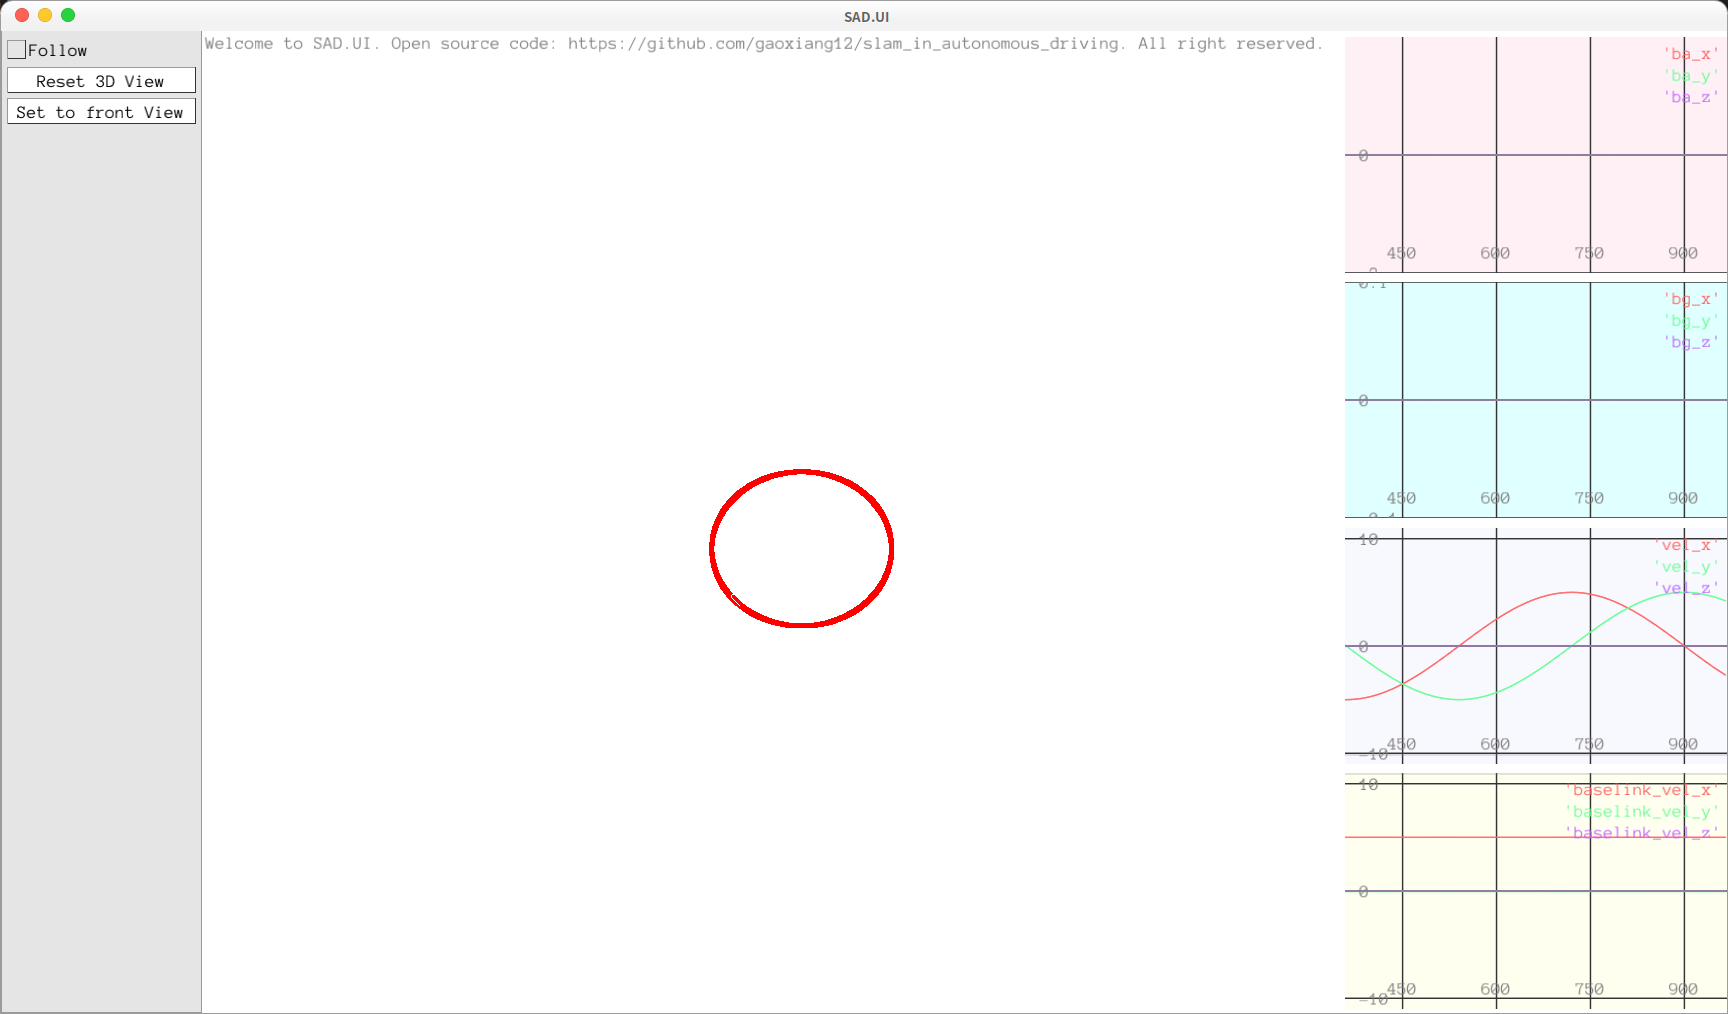
\includegraphics[width=0.7\textwidth]{math-basics/motion-example.png}
%	\caption{一个圆周运动车辆的运动学模拟}
%	\label{fig:motion-example}
%\end{figure}
%
%本书后文的大部分程序都可以通过这种方式执行。读者可以用本节程序来适应一下本书的代码风格。通过本节实验,我们可以看到车辆走出一个完整的圆形轨迹,它的世界系速度类似于三角函数,本体系下速度则保持$X$轴固定不变。使用四元数还是旋转矩阵,在处理运动学方面并无本质差异。读者可以利用本节程序,演示一些常见的自由落体或者抛物线运动。这些作为本节习题留给读者。
%
%\section{滤波器与最优化理论}
%下面我们回顾基础的滤波器原理以及它和最优化方法之间的联系。我们仍然从状态估计讲起。
%
%\subsection{状态估计问题与最小二乘}
%SLAM问题、定位问题或者建图问题都可以概括为状态估计问题。典型的离散时间状态估计问题由一
%组运动方程和一组观测方程组成:
%\begin{equation}
%	\left\{ \begin{array}{l}
%		{\mathbf{x}_k} = \mathbf{f}\left( {{\mathbf{x}_{k - 1}},{\mathbf{u}_k}} \right) + \mathbf{w}_k,\quad k=1, \ldots, N\\
%		{\mathbf{z}_{k}} = \mathbf{h} \left( \mathbf{x}_k  \right)+ \mathbf{v}_{k},
%	\end{array} \right.
%\end{equation}
%其中$\mathbf{f}$称为运动方程,$\mathbf{h}$称为观测方程,$\mathbf{w}_k \sim \mathcal{N}(\mathbf{0}, \mathbf{R}_k)$, $\mathbf{v}_k 
%\sim \mathcal{N}( \mathbf{0}, \mathbf{Q}_k)$为高斯分布的随机噪声。如果设$\mathbf{f}$和$\mathbf{h}$为线性函数,就可以得到线性高斯系统(linear Gaussian, LG系统)的状态估计问题:
%\begin{equation}
%	\left\{ \begin{array}{l}
%		{\mathbf{x}_k} = \mathbf{A}_k {{\mathbf{x}_{k - 1}}+{\mathbf{u}_k}} + \mathbf{w}_k \\
%		{\mathbf{z}_{k}} = \mathbf{C}_k  { \mathbf{x}_k} + \mathbf{v}_{k} \end{array} \right. .
%\end{equation}
%其中$\mathbf{A}_k, \mathbf{C}_k$为系统的转移矩阵和观测矩阵。线性系统是最简单的状态估计问题,它的
%无偏最优估计由\textbf{卡尔曼滤波器}(Kalman filter, KF)给出\cite{Zarchan2005,Barfoot2016}。
%
%\subsection{卡尔曼滤波器}
%卡尔曼滤波器描述了如何从一个时刻的状态估计递推到下一个时刻。它由\textbf{预测}(prediction)和\textbf{更新}(update)两个步骤组成。预测步骤对运动方程进行递推,观测步骤则对上一步结果进行修正。我们设$k-1$时刻状态估计为$\mathbf{x}_{k-1},
% \mathbf{P}_{k-1}$,其中$\mathbf{x}_{k-1}$为均值,$\mathbf{P}_{k-1}$为估计协方差矩阵。
%\begin{mdframed}
%	\begin{enumerate}
%		\item 预测:
%		\begin{equation}
%			\mathbf{x}_{k,\mathrm{pred}} = {\mathbf{A}_k {\mathbf{x}_{k - 1}} + {\mathbf{u}_k}}, \quad 
%			\mathbf{P}_{k,\mathrm{pred}} = \mathbf{A}_k \mathbf{P}_{k-1} \mathbf{A}^\top_k + \mathbf{R}_k.
%		\end{equation}
%		\item 更新:
%		先计算$\mathbf{K}$,它又称为\textbf{卡尔曼增益}。
%		\begin{equation}
%			\label{eq:kalman-K-another}
%			\mathbf{K}_k = \mathbf{P}_{k, \mathrm{pred}} \mathbf{C}_k^\top {\left( {\mathbf{C}_k \mathbf{P}_{k, 
%			\mathrm{pred}} \mathbf{C}_k^\top + {\mathbf{Q}_k}} \right)^{ - 1}}.
%		\end{equation}
%		然后计算后验概率的分布。
%		\begin{equation}
%			\begin{array}{l}
%				{\mathbf{x}}_k = {\mathbf{x}_{k, \mathrm{pred}}} + \mathbf{K}_k \left( {\mathbf{z}_k - 
%				{\mathbf{C}_k}{\mathbf{x}_{k, \mathrm{pred}}}} \right), \\
%				\mathbf{P}_k = \left( {\mathbf{I} - \mathbf{K}_k {\mathbf{C}_k}} \right) \mathbf{P}_{k, \mathrm{pred}}.
%			\end{array}
%		\end{equation}
%	\end{enumerate}
%\end{mdframed}
%
%其中下标$\text{pred}$表示预测得到的结果。不同书籍可能会使用各种不同的符号来表达它和最终估计值的差异,比如$\hat{\mathbf{x}}, \mathbf{x}^*, \check{\mathbf{x}}$,等等。本书后文统一使用下标方式来区分预测变量。
%
%我们不准备展开线性卡尔曼滤波器的推导过程。但我们要提醒读者,在线性系统中,各类方法(贝叶斯滤波、卡尔曼滤波、最小二乘、增益最优化等)都会达成同样的结论,“条条大路通罗马”,所以卡尔曼滤波器可以由各种方法推导出来,例如:
%\begin{enumerate}
%	\item 从增益最优化角度来推导,即,假设最优估计由$\mathbf{x}_{k, \mathrm{pred}} +\mathbf{K}_k (\mathbf{z}_k - \mathbf{C}_k \mathbf{x}_{k, \mathrm{pred}})$形式构成,然后寻找最优的$\mathbf{K}_k$。这种推导方式最为简单,也是大多数
%	类似材料的首选推导方法。
%	\item 从贝叶斯滤波器来推导,这需要用到高斯分布的线性变换和边缘化。这也是\cite{Thrun2005}
%	的首选做法,也是我们在《十四讲》中的做法。
%	\item 从最大后验估计(MAP)来推导,这种方法只需要基础的线性代数即可。 
%	\item 
%	从批量MAP解出发,使用Cholesky分解区分前后向过程,由前向过程推导卡尔曼滤波。这是\cite{Barfoot2016}
%	的首选做法,优点是可以很好地显示卡尔曼滤波器与Rauch-Tung-Stribel Smoother(RTS平滑)方法的联系(
%	以及与批量MAP间的联系),缺点是推导过程比较复杂,需要大量的篇幅。
%\end{enumerate}
%
%与传统卡尔曼滤波器不同的是,本书会统一使用李群李代数的方式来处理卡尔曼滤波器。因为我们需要考虑运动学方程,所以状态变量$\mathbf{x}$除了含有位置和姿态以外,还会带有速度、传感器零偏等其他变量。这样一个高维的$\mathbf{x}$就落在一个高维流形$\mathcal{M}$上,称为\textbf{流形上的卡尔曼滤波器}(KF on manifold)\cite{he2021kalman}。在下一章我们会看到,这种流形的处理方式要比基于欧拉角或者四元数原始分量的方式更加简洁。
%
%\subsection{非线性系统的处理方法}
%在非线性系统中,首选的方式是对$\mathbf{f}$和$\mathbf{h}$进行\textbf{线性化}(linearization)。线性化本质是求一个函数在固定点的\textbf{泰勒展开}(Taylor expansion),并保留一阶系数。线性化是后文广泛用到的理论。如果对一个普通的矢量函数$\mathbf{f}(\mathbf{x})$在$\mathbf{x}_0$点处进行线性化,应该得到:
%\begin{equation}\label{key}
%\mathbf{f} (\mathbf{x}_0 + \Delta \mathbf{x}) = \mathbf{f} (\mathbf{x}_0) + \mathbf{J} \Delta \mathbf{x} + \frac{1}{2} \Delta \mathbf{x} ^\top \mathbf{H} \Delta \mathbf{x} + O(\Delta \mathbf{x}^2),
%\end{equation}
%这里$\mathbf{J}$称为\textbf{雅可比矩阵}(Jacobians),$\mathbf{H}$称为\textbf{海塞矩阵}(Hessians),是线性化中最重要的两个矩阵。如果只保留一阶项,那么$\mathbf{f}(\mathbf{x})$就可以近似为:
%\begin{equation}\label{key}
%\mathbf{f} (\mathbf{x}_0 + \Delta \mathbf{x}) \approx \mathbf{f} (\mathbf{x}_0) + \mathbf{J} \Delta \mathbf{x},
%\end{equation}
%
%我们可以对非线性系统的运动方程和观测方程进行线性化,然后将卡尔曼滤波器的结论应用在非线性系统中,得到\textbf{扩展卡尔曼滤波器}(Extended Kalman filter, EKF)。如果不展开讨论$\mathbf{x}$的定义以及各矩阵的详细形式,通用的EKF可以简单描述如下。
%
%首先,将运动方程在上一时刻的状态进行线性化,得到:
%\begin{equation}\label{key}
%\mathbf{x}_k \approx \mathbf{f}(\mathbf{x}_{k-1}, \mathbf{u}_k) + \mathbf{F}_k \Delta \mathbf{x}_k + \mathbf{w}_k,
%\end{equation}
%这里$\mathbf{F}$即为运动方程的相对于上一时刻状态的雅可比矩阵。该矩阵主要用于计算协方差的预测值。至于均值的预测值,可以将$\mathbf{x}_{k-1}$代入$\mathbf{f}$后得到。这样就写出了EKF的预测过程:
%\begin{mdframed}
%\begin{equation}\label{key}
%\mathbf{x}_{k, \text{pred}} = \mathbf{f}(\mathbf{x}_{k-1}, \mathbf{u}_k), \quad \mathbf{P}_{k, \text{pred}} = \mathbf{F}_k \mathbf{P}_{k-1} \mathbf{F}_k^\top + \mathbf{R}_k.
%\end{equation}
%\end{mdframed}
%注意这里实际上假设了\textbf{一个高斯分布状态变量经过非线性函数后仍为高斯分布}。这其实是一个近似,与实际情况可能差别较大。对于观测方程,可以在$\mathbf{x}_{k, \text{pred}}$处作线性化,得到:
%\begin{equation}\label{key}
%\mathbf{z}_k \approx \mathbf{h}(\mathbf{x}_{k, \text{pred}}) + \mathbf{H}_k (\mathbf{x}_k - \mathbf{x}_{k, \text{pred}}) + \mathbf{n}_k,
%\end{equation}
%然后代入卡尔曼滤波器的增益公式和更新方程,就可以得到EKF的更新过程:
%\begin{mdframed}
%\begin{align}\label{key}
%\mathbf{K}_k &= \mathbf{P}_{k, \text{pred}} \mathbf{H}_k^\top (\mathbf{H}_k \mathbf{P}_{k, \text{pred}} \mathbf{H}_k^\top + \mathbf{Q}_k)^{-1}, \\
%\mathbf{x}_k &= \mathbf{x}_{k, \text{pred}} + \mathbf{K}_k (\mathbf{z}_k - \mathbf{H}_k \mathbf{x}_{k, \text{pred}}), \\
%\mathbf{P}_k &= (\mathbf{I} - \mathbf{K}_k \mathbf{C}_k) \mathbf{P}_{k, \text{pred}}.
%\end{align}
%\end{mdframed}
%
%对比KF和EKF,我们发现它们在公式上基本是一样的,只是EKF几个系数矩阵并不固定,可以随着线性化点发生改变而已。
%
%这样我们就快速地回顾了一遍KF和EKF的公式,但这里的讨论并没有展开说明,当$\mathbf{x}$中存在位移、旋转、速度等变量时,每个矩阵应该怎样计算。特别地,如果$\mathbf{x}$当中的旋转以$\mathbf{R}$的形式来表示,我们实际并不能直接写$\mathbf{x}_k - \mathbf{x}_{k-1}$或者$\mathbf{x}_k - \mathbf{x}_{k, \text{pred}}$这样的写法,而应该使用左右扰动模型来处理这些项。当引入李群李代数之后,EKF应该作出怎样的改变,是我们在第~\ref{cpt:ins}~章中要讨论的问题。
%
%\subsection{最优化方法与图优化}
%另一方面,运动学方程和观测方程都可以看成一个状态变量$\mathbf{x}$与运动学输入、观测值之间的残差,这是一种\textbf{批量最小二乘}(batch least square)的视角:
%\begin{align}\label{eq:2.118}
%\mathbf{e}_{\text{motion}} &= \mathbf{x}_k - \mathbf{f}(\mathbf{x}_{k-1}, \mathbf{u}) \sim \mathcal{N}(\mathbf{0}, \mathbf{R}_k), \\
%\mathbf{e}_{\text{obs}} &= \mathbf{z}_k - \mathbf{h}(\mathbf{x}_k) \sim \mathcal{N}(\mathbf{0}, \mathbf{Q}_k).
%\end{align}
%
%而滤波器当中的最优状态估计可以看成关于各误差项的最小二乘问题:
%\begin{equation}\label{key}
%\mathbf{x}^* = \arg \min_{\mathbf{x}}  \sum_{k} \left( \mathbf{e}_k^\top \boldsymbol{\Omega}_k^{-1} \mathbf{e}_k \right).
%\end{equation}
%其中$\mathbf{e}_k$表示第$k$项误差,$\boldsymbol{\Omega}_k$为该误差的协方差矩阵。这里$\mathbf{e}_k$可以由前面的运动误差或观测误差代入,但最小二乘算法并不刻意区分运动学误差或观测误差。对于一个通用的误差函数$\mathbf{e}_k$组成的最小二乘问题,我们可以用\textbf{迭代最优化}方法进行求解。它们的整体思路是这样的:
%
%\begin{enumerate}
%\item 首先,从$\mathbf{x}$的某个初始值出发,例如$\mathbf{x}_0$。
%\item 设第$i$次的迭代值为$\mathbf{x}_i$,那么对上述误差函数,在$\mathbf{x}_i$处进行线性化,得到:
%\begin{equation}\label{key}
%\mathbf{e}_k(\mathbf{x}_i + \Delta \mathbf{x}) \approx \mathbf{e}_k (\mathbf{x}_i) + \mathbf{J}_{k,i} \Delta \mathbf{x}_i ,
%\end{equation}
%这里线性化矩阵为$\mathbf{J}_{k,i}$。
%\item 利用高斯牛顿法或者类似的求解方法,解得本次迭代的增量$\Delta \mathbf{x}_i$。以高斯牛顿法为例,其求解的线性方程为:
%\begin{equation}\label{key}
%\sum_k (\mathbf{J}_{k,i} \boldsymbol{\Omega}_k^{-1} \mathbf{J}_{k,i}^\top) \Delta \mathbf{x}_i = - \sum_k (\mathbf{J}_{k,i} \boldsymbol{\Omega}_k^{-1} \mathbf{e}_k).
%\end{equation}
%\item 更新$\mathbf{x}_i$,得到下次迭代值:$\mathbf{x}_{i+1} = \mathbf{x}_i + \Delta \mathbf{x}_i$。
%\item 判断算法是否收敛。若收敛则退出,不收敛则进行下一次迭代。
%\end{enumerate}
%
%最优化方法与滤波器方法有千丝万缕的联系。它们在线性系统中会得到同样的结果\cite{Barfoot2016},但在非线性系统中通常不然。主要原因有以下几个:
%\begin{enumerate}
%	\item 最优化方法有迭代过程,而EKF则没有。
%	\item 迭代过程会不断在新的线性化点$\mathbf{x}_i$上求取雅可比矩阵,而EKF的雅可比矩阵只在预测位置上求取一次。
%	\item EKF还会区分$\mathbf{x}_{k,\mathrm{pred}}$,分开处理预测过程与观测过程。而最优化方法则没有$\mathbf{x}_{k,\mathrm{pred}}$,统一处理各处的状态变量。
%\end{enumerate}
%
%一个重要的问题是,如果我们忽略上述第3条,将卡尔曼滤波器看作非线性优化,那么卡尔曼滤波器应该有几个优化变量和几种误差函数?答案是:两个优化变量,三种误差函数。两个优化变量是指$\mathbf{x}_{k-1}$和$\mathbf{x}_{k}$,而三种误差函数分别是:
%\begin{enumerate}
%\item $k-1$时刻的状态$\mathbf{x}_{k-1}$服从它的先验高斯分布。我们设$\mathbf{x}_{k-1} \sim \mathcal{N}(\bar{\mathbf{x}}_{k-1}, \mathbf{P}_{k-1})$\footnote{注意这里必须引入$\bar{\mathbf{x}}_{k-1}$,它是一个已知的数值,在上一时刻算得。而$\mathbf{x}_{k-1}$是一个可变化的变量,请注意区分。},那么此处产生了一个\textbf{先验误差}:
%\begin{equation}\label{key}
%\mathbf{e}_{\text{prior}} = \mathbf{x}_{k-1} - \bar{\mathbf{x}}_{k-1} \sim \mathcal{N}(0, \mathbf{P}_{k-1}).
%\end{equation}
%\item 从$k-1$到$k$的\textbf{运动误差};
%\item $k$时刻的\textbf{观测误差}。
%\end{enumerate}
%后两者已经列写在式\eqref{eq:2.118}中。这样,卡尔曼滤波器与最优化问题就等效了起来(见图~\ref{fig:ekf-factors})。当然它们实际求解过程是有差异的。EKF并不会更新$\mathbf{x}_{k-1}$,只计算$\mathbf{x}_k$的变化量,而最优化则一视同仁。另一方面,EKF也会更新协方差矩阵$\mathbf{P}_{k}$,而普通的优化器只计算均值部分$\mathbf{x}_{k}$。如果我们想得到$\mathbf{P}_{k}$,还需要对最优化问题进行\textbf{边缘化}(Marginalization)。
%
%\begin{figure}[!htp]
%	\centering
%	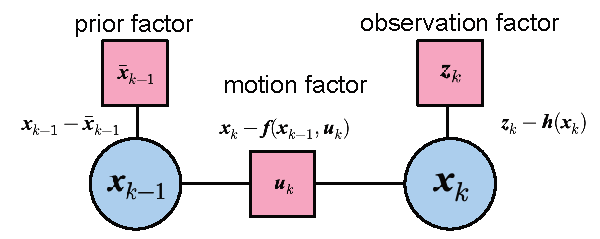
\includegraphics[width=0.7\textwidth]{math-basics/ekf-factors.pdf}
%	\caption{卡尔曼滤波器与图优化模型}
%	\label{fig:ekf-factors}
%\end{figure}
%
%在SLAM领域,最优化问题通过用图模型进行描述,对应的图模型称为\textbf{图优化}(graph optimization)或者\textbf{因子图}(factor graph)。因子图模型可以进一步引入\textbf{概率图模型}中的方法进行求解。本书不刻意区分图优化和因子图的概念,它们在实际操作当中通常没有太大区别。但是,将卡尔曼滤波器与图优化方法进行对比和讨论,是本书后文的重点之一。我们会实际来实现一遍经典的EKF和图优化方法,来求解带有惯导、GPS和激光点云的问题。我们也会将EKF拓展成迭代卡尔曼滤波器(IEKF),来处理观测模型中存在最近邻问题的情况(带有最近邻问题的观测模型,方程数量和形式可能在迭代过程中发生改变,而非简单地在不同点进行线性化)。
%
%\section{小结}
%本节向读者介绍了常见的各种坐标系、运动学理论,重点介绍了四元数与$\mathrm{SO}(3)$两种处理运动学的方法,并讨论了它们的异同。我们也回顾了KF、EKF的基本公式,讨论了它们和图优化之间的一些差异。
%
%本节内容以回顾为主,下一节我们将展开介绍ESKF,并给出实现以及动画演示。
%
%\section*{习题}
%\begin{enumerate}
%	\item 分别使用左右扰动模型,计算 $$\frac{\partial \mathbf{R}^{-1} \mathbf{p}}{\partial \mathbf{R}}.$$
%	\item 分别使用左右扰动模型,计算 $$\frac{\partial \mathbf{R}_1 \mathbf{R}_2^{-1}}{\partial \mathbf{R}_2}.$$
%	\item 将\ref{sec:motion-example}节的实验修改成带旋转的抛物线运动。物体一方面沿Z轴自转,一方面存在水平的初始线速度,又受到$-Z$方向的重力加速度影响。请设计程序并完成动画演示。
%\end{enumerate}

\newpage
 
\addtocontents{toc}{\protect\setcounter{tocdepth}{2}}
\hypersetup{bookmarksdepth=2}

\appendix
\addtocontents{toc}{\protect\setcounter{tocdepth}{0}}
\hypersetup{bookmarksdepth=2}

%\input{chapters/gaussian-distribution}
%\input{chapters/matrix-derivatives}

\backmatter
\small
\bibliographystyle{ieeetr}
\bibliography{ref}
\newpage
\end{document}
